\documentclass[a4paper,twoside,12pt]{kth-mag}
\usepackage[english]{babel}   % automated words (as titles) in english
\usepackage[T1]{fontenc}
\usepackage[latin1]{inputenc} % it will permit us write using latin1 (tildes..)
\usepackage{lmodern}          % nice fonts
\usepackage{listings}
\usepackage{graphicx}
\usepackage{enumerate}
\usepackage{xspace}  % used in the reflect icon
\usepackage{color}   % defining colours
\usepackage{nada-ex} % KTH Nada exjobb customizations
\usepackage{lscape}  % landspace pages
%\usepackage{draftwatermark} % draft symbols
\usepackage{amsfonts} % mathematical fonts
\usepackage{subfig}
\usepackage[pdftitle={Hardware synthesis in ForSyDe},
            pdfauthor={Alfonso Acosta},
            pdfsubject={Compilers},
            pdfkeywords={Alfonso Acosta, Masther's Thesis, ForSyDe,
              thesis report, KTH, Lava, Haskell, VHDL, Compiler,
              embedded compiler, DSL, EDSL, alfonso.acosta@gmail.com,
              functional programming},
            pdfstartview=Fit, % fullscreen when opening
            %pdfview=FitB, % FIXME!!
            pdfpagemode=UseOutlines, % show outlines
            pdfpagelayout=OneColumn, % 
            bookmarksopen=false, % despliegue del indice
            colorlinks=true, 
            linkcolor=black,
            urlcolor=black,
            citecolor=black,
            breaklinks=true 
           ]
           {hyperref}       
\usepackage{xmpincl} % include licensing metadata
\usepackage{longtable}

%%%%%
% Front page information
%%%%%

\title{Hardware synthesis in ForSyDe}
\subtitle{The design and implementation of a\\ ForSyDe-to-VHDL Haskell-embedded compiler}

\author{Alfonso Acosta} 

\date{June 2007}

\trita{}%{TRITA xxx yyyy-nn}

\blurb{Master's Thesis at KTH/ICT/ECS\\Supervisor: Ingo Sander\\Examiner: Ingo Sander\\Stockholm, \thedate}


%%%%%%
% Commands used through the thesis
%%%%%%

%signals, used in Ingo's figures
\newcommand{\signal}[1]{$\overrightarrow{#1}$}

\newcommand{\reFLect}{\textit{re\kern-0.07em
    F\kern-0.07emL\kern-0.29em\raisebox{0.56ex}{ect}}\xspace}

%%%%%%
% Settings
%%%%%%

% where to look for graphics

\graphicspath{{figures/}}

% logo used in the main page
\kthlogo{kth_svv}

% grey for the listings
\definecolor{gris}{gray}{0.95}

% settings for the listings
\lstset{language=Haskell,
  linewidth=\linewidth,
  stringstyle=\ttfamily,
  basicstyle=\scriptsize\ttfamily,
  frame=single,
  frameround=tttt,
  backgroundcolor=\color{gris}}

% licensing metadata
\includexmp{CC_Attribution-No_Derivative_Works_3.0}

%%%%%%
% Document skeleton
%%%%%%

\begin{document}
\begin{titlingpage}
\maketitle

\begingroup
\vspace*{\fill}
\footnotesize
\setlength{\parindent}{0pt}
\setlength{\parskip}{\baselineskip}
Copyright \textcopyright{} 2007 by Alfonso Acosta <\href{mailto:alfonso.acosta@gmail.com}{\nolinkurl{alfonso.acosta@gmail.com}}>

This work is licensed under the Creative Commons Attribution-No
Derivative Works 3.0 License. To view a copy of this license, visit
\url{http://creativecommons.org/licenses/by-nd/3.0/} or send a letter
to Creative Commons, 171 Second Street, Suite 300, San Francisco,
California, 94105, USA.
\endgroup
\end{titlingpage}
 
\frontmatter
\chapter{Abstract}


The ForSyDe (\textit{Formal System Design}) methodology
is targeted at modelling systems, with the goal of using a high level
of abstraction in the specification of its models.

Although it is a general system modelling methodology, the initial
scope of ForSyDe has specifically been \textit{Synchronous Systems}
(systems in which a global clock is used to synchronize the different
parts of the system). A well-known type of such system is synchronous
hardware, which is the main subject of this thesis. A synchronous
system in ForSyDe is based on the concept of \textit{processes} which
\textit{``map input signals onto output signals''}.

Currently, the software implementation of ForSyDe is based upon the
Haskell programming language. The designer specifies the
system model in Haskell as a network of cooperating process
constructors with the assistance of the ForSyDe Library.

Until now, there has not been an automated way to synthesize ForSyDe
models (i.e.  generate an equivalent low-level implementation from
which to build real hardware) .  However, as a result of this thesis,
hardware synthesis is now a feature of ForSyDe, enabling ForSyDe
designs to finally reach silicon.  That is possible thanks to the
development of a ForSyDe-to-VHDL compiler.  By using this compiler, a
ForSyDe model can be first translated to synthesizable
VHDL93 (one of the two most common hardware design
languages) and then, the designer can use any of the existing
VHDL-tools to synthesize the model.

This thesis report is aimed at documenting the background, design,
implementation and use of the compiler.


\chapter{Acknowledgements}
There are many people who in one form or another contributed to the work
described in this thesis. 

I would like to thank Ingo Sander, my supervisor, for his flexibility
and trust during the thesis.  He has always been positive about my,
sometimes not-so-frequent and too extensive, thesis status reports. I
would also like thank him and give him credit for kindly letting me
use some of the figures of his PhD thesis \cite{forsyde:thesis}.

I am also tremendously thankful to the Haskell community, which has proven to
be, by far, the most friendly, helpful and smart programming community I have
ever been involved with. Special thanks go to the guys at the
\texttt{\#haskell} IRC channel at \texttt{freenode.net} and the
\texttt{haskell-cafe} mailing list. There are too many community-people to
thank but I would like to specifically mention Oleg Kiselyov for his selfless
help fixing and designing the compiler's typechecker.

Koen Claessen gave me access to Lava's sourcecode, which turned to be essential
during the developmnent of the compiler. Without Lava, the compiler would
have been totally different and perhaps even unfeasible.

Last but not least, I would like to thank Iv\'{a}n P\'{e}rez and
Miguel Jim\'{e}nez who helped reviewing parts of the thesis, my
parents, for their support, whithout which I would not had been able
to spend my last two academic years in Stockholm and finally, all the
Erasmus students which turned my stay in Sweden into one of the best
experiences of my life (they know who they are).

\vspace{\baselineskip} 
\noindent Stockholm, \thedate

\vspace{\baselineskip} 
\noindent\theauthor

\chapter{Preface}
This thesis report is aimed at documenting the background, design,
implementation and use of a compiler which translates ForSyDe (\textit{Formal
  System Development}) specifications into VHDL93 \cite{vhdl93} synthesizable
code.

The current implementation of ForSyDe, in which the compiler was embedded,
is written in the Haskell \cite{haskell} programming language. That
means the compiler has unavoidably been coded in the same
language. For that reason, \textbf{it will be assumed that the reader
of this report is fluent in Haskell}. Introducing the reader to
Haskell is out of the scope of the present text. There are many
resources from where to acquire the necessary knowledge. Just to
mention three of them, \textit{A Gentle Introduction to
Haskell} \cite{haskellgentle} is available online at no cost and is
supposed to be a friendly text for the newcomers, Thomson's book
\textit{Haskell: the Craft of Functional Programming} \cite{craft} on
the other hand is longer but covers the language in greater detail and
finally the upcoming \textit{Real-World Haskell} book\footnote{Not
ready by the time of writing this preface.} \cite{realworldhaskell}
will be freely available online and will help to get involved with
serious real-world Haskell code and practical Haskell
programming. Mastering Haskell is not a prerequisite to understand the
overall content of the thesis. However, wide Haskell
programming-experience and familiarity with its common extensions
would definitively be useful (and is probably needed) to comprehend
the compiler's design and implementation details.

In addition, it will be assumed that the reader is familiar with
digital hardware design and development through HDLs (\textit{Hardware
Design Languages}) or, in the worst case, understands the concepts
behind it. This prerequisite is weaker than knowing Haskell, since
specific knowledge of VHDL is not essential to read the
report. However, being aware of the purpose of an HDL is vital to
understand the goals which were achieved.

This thesis report is divided in five chapters:

\textbf{Chapter \ref{chap:intro}} introduces the reader to ForSyDe and
the thesis goals. It also introduces the concept of Embedded DSL
(\textit{Domain Specific Language}) which is essential to understand
ForSyDe's implementation.

\textbf{Chapter \ref{chap:vs}} is targeted at comparing ForSyDe with
Lava, a successful Haskell-embedded HDL (\textit{Hardware Description
Language} ) and verification environment. The comparison was written
before developing the compiler, in order to acquire the necessary
background in the \textit{Hardware Design and Functional Languages}
research field, hoping to be able to later reuse previous research
results and provide ForSyDe's compiler with state-of-the-art features.

ForSyDe's translator to VHDL turned out to be strongly influenced by
Lava. As a result of the comparison, the compiler is intended to
inherit Lava's virtues and overcome some of its problems such as its
current lack of component reusability on the
compiler-level. \textbf{Chapter \ref{chap:design}} describes the
design of the compiler and the motivation behind it whereas
\textbf{Chapter \ref{chap:user}} is targeted at the end-user and
contains a tutorial to help getting familiar with the tool and its
API.

Finally \textbf{Chapter \ref{chap:conc}} closes the thesis analyzing
its results and outlining potential improvements and further work.

As an add-on, \textbf{appendix \ref{chap:hacker}} has been written with future
developers in mind. They will surely find this appendix useful to get
familiar with the compiler's implementation in first instance, and
later improve it or extend it at will (the sources are available under
the BSD licence at
\url{http://www.imit.kth.se/info/FOFU/ForSyDe/HDForSyDe/}).

\clearpage
\tableofcontents
\clearpage
\listoffigures
\clearpage
\chapter{List of Abbreviations}
\begin{longtable}{p{.2\textwidth}p{.8\textwidth}}
ADT & Abstract Data Type \\
API & Application Programming Interface\\
AST & Abstract Syntax Tree\\
BSD & Berkeley Software Distribution\\
CAD & Computer-Aided Design\\
DSL& Domain Specific Language\\
EDSL & Embedded DSL\\
ForSyDe & Formal System Design \\
FPGA& Field-Programmable Gate Array\\
GHC & Glasgow Haskell Compiler\\
HDL & Hardware Description Language\\
IO & Input Output\\
IRC & Internet Relay Chat\\
MPTC & Multi-parameter Type Class\\
RTL & Register Transfer Level\\
ST & State Transformer \\
TH& Template Haskell\\
VHDL & VHSIC HDL\\
VHSIC & Very-High-Speed Integrated Circuit\\
VLSI & Very-Large-Scale Integration \\
XML & eXtensible Markup Language\\
YACC & Yet Another Compiler Compiler\\
\end{longtable}
\clearpage
\mainmatter



\chapter{Introduction}
\label{chap:intro}

\section{Introduction}
\label{sec:Introduction}

\cite{SanJan2004a}

\cite{BjeCla1998}


\chapter{Lava vs ForSyDe}
\label{chap:vs}
This chapter is aimed at comparing Lava and ForSyDe, two DSLs (\textit{Domain
  Specific Languages}) embedded in Haskell.  The comparison was made at the
initial stage of the thesis, as a means of acquiring a picture of the previous
work in the Functional Programming and Hardware Description field, in order to
hopefully reuse earlier design techniques and to provide ForSyDe's compiler
with state-of-the-art features. Thus, at the time of writing this comparison
the compiler was not yet designed.


  During the comparison, the reader will get familiar with the
  important concept of \textit{Embedded Compiler}. Furthermore, by the end
  of the chapter he (or she) will ...  

  \begin{itemize}
  \item  ... be able to understand the problems
    related to represent circuits in a purely functional programming
    language such as Haskell.
  \item ... hopefully have acquired a valuable background
    in the Hardware design and Functional Languages field along with
    an up-to-date view of the previous work related to this thesis.
  \end{itemize}

  \section{Introduction}
  The complexity of electronic designs has tremendously risen during the past
  two decades which, together with the Industry's exigency of extremely
  short time-to-market periods have made RTL-level tools no longer fit
  nowadays circuit design requirements. Thus, there has been a
  natural move to a higher level of abstraction known as
  \textit{System Level Design}.

  The two most commonly-used RTL-level HDLs (Verilog and VHDL) are far
  too verbose and concrete to cleanly give a general view of a
  complex system.

  Therefore, new languages are needed to provide a solution for the
  aforementioned problems.  Among other approaches which require
  creating a new programming language from scratch, the
  \textit{Embedded Approach} saves the designer having to learn a new
  syntax and makes possible to reuse all the existing tools (i.e.
  compilers, interpreters ...)  surrounding the \textit{host
    language}.

  Furthermore, the expressiveness of declarative languages such as
  Haskell seems to suit the abstraction level of \textit{System Level
    Design}  \cite{declarative} and hardware design semantics
   \cite{funhw}.

  During the rest of this chapter, two Haskell-embedded language
  approaches will be compared: Lava \cite{lava} and
  ForSyDe \cite{forsyde}. The later targets synchronous systems in
  general (that is, systems in which a single global clock is
  used\footnotemark \footnotetext{ForSyDe supports as well a
    \textit{multi-rate model} by using \textit{multi-rate interfaces},
    able to connect different synchronous sub-domains working at
    different clock rates.}), while the first specifically describes
  synchronous hardware (a concrete type of synchronous system after
  all) and is the most mature of the two.
  
\section{Design flow}
Lava and ForSyDe were independently developed by the Swedish
universities of Chalmers and KTH.

Figures \ref{fig:lava} and \ref{fig:forsyde} contain diagrams
describing the simplified design flow to be followed when modelling with
Lava and ForSyDe.  As it will be later seen, the flow is quite
similar to the traditional compilation model of a
general-purpose programming language.

It is easy to suspect that both Lava and ForSyDe follow a similar
approach, sequentially divided in two stages:


\begin{enumerate}[1)]
  \item The designer models a circuit in Haskell, making use
    of the Lava or ForSyDe libraries.



  \item The obtained model is automatically processed by a compiler in
    order to attain different \textit{goals}: simulation, testing,
    verification and translation to a less abstract HDL (e.g. VHDL)
    directly synthesizable to hardware. The different flavours of this
    stage are known as \textit{Interpretations} in Lava and
    \textit{Implementation Mappings} in ForSyde. In the rest of this
    chapter I will refer to them with the wider spread term:
    \textit{backends}.  The details of these backends will be
    described in next section.


\begin{landscape}
  \begin{figure}
    \centering
    \begin{minipage}[t]{.45\linewidth}
      \caption{Lava's design flow}\label{fig:lava}
      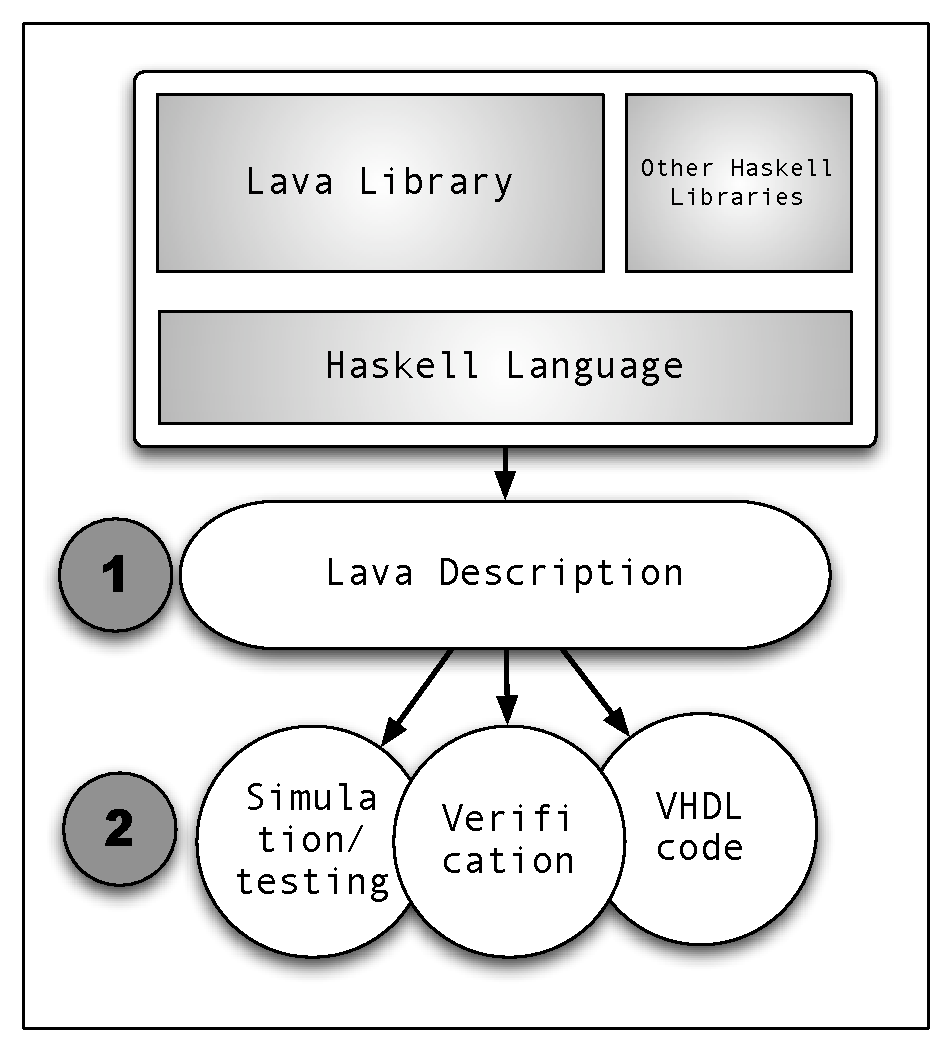
\includegraphics[width=\linewidth]{Lava.pdf}
    \end{minipage}
    \hfil
    \begin{minipage}[t]{.45\linewidth}
      \centering
      \caption{ForSyDe's design flow}\label{fig:forsyde}
      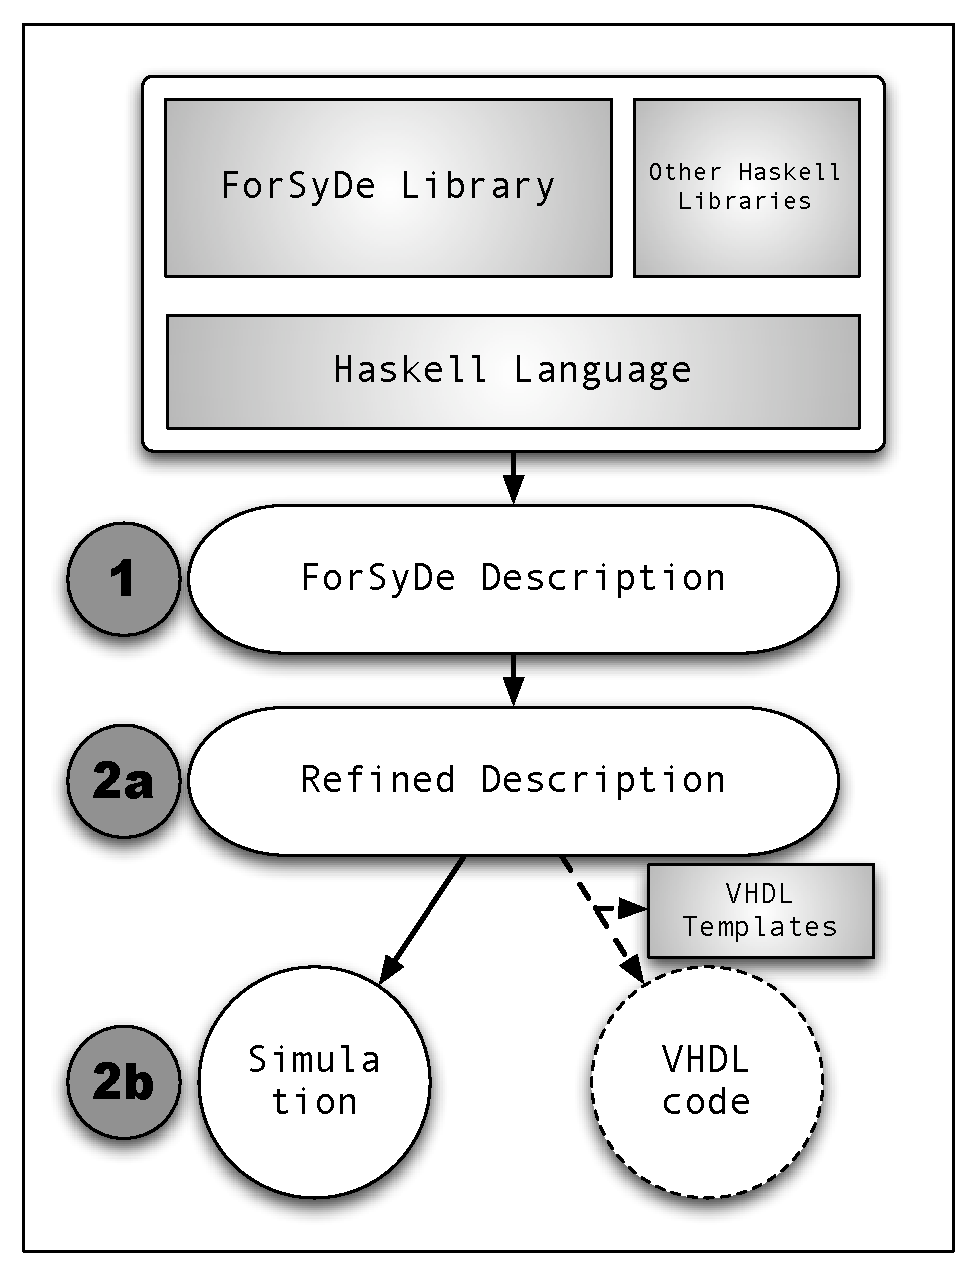
\includegraphics[width=\linewidth]{ForSyDe.pdf}
    \end{minipage}
  \end{figure}
\end{landscape}


    This stage slightly differs depending on the language used, being more
    complex, and potentially more likely to include optimizations in
    the case of ForSyDe, due to the application of \textit{Design
      Transformations}.
    
    ForSyDe has a strong formal base which allows the designer to work
    at a highly abstract functional level. The abstraction level is
    lowered\footnote{ForSyDe currently lacks an automatic tool
      for this purpose and transformations need to be applied
      manually. Either the case,  \cite{forsyde:thesis} proves it would not
      only feasible but quite straight-forward to implement.} by
    applying \textit{Transformation Rules} to the provided hardware
    descriptions. That is captured in figure \ref{fig:forsyde} as the
    transition from 2a to 2b.

    The internal details of  ForSyDe's \textit{Refinement} are out of
    the scope of this chapter but is worth to mention that the
    \textit{Transformation Rules} can be divided in \textit{semantic
      preserving} and \textit{design decisions}. The later ones
    change the semantics of the model and thus, its application must be
    supervised by the designer.
\end{enumerate}
\section{Backends}
As it was mentioned previously, Lava is in a more mature state than
ForSyDe, having a whole set of tools surrounding it.

On the other hand, ForSyDe only currently supports simulation by
direct execution of its Haskell models\footnote{\textit{Zero-delays},
  circuit feedback loops without delays, are forbidden in ForSyDe and
  thus cannot be simulated.}. Even with that, a \textit{template
  system}, in which every library function has a preassigned VHDL
template, has been already planed and a few prove-of-concept
examples \cite[Chapter 6]{forsyde:thesis} back it as a promising
approach.

As of the time of writing this thesis, Lava has three available backends:

\begin{itemize}
\item \textbf{Simulation and random testing}. A circuit simulation
  is carried out by interpreting each component of its
  structure\footnote{Zero-delays are only permitted when performing a
    \textit{constructive} simulation by using \texttt{simulateCon},
    see Lava's documentation \cite{lava:thesis} for details.}.

  In addition, Lava allows to test properties of a
  design on random data through a language which is highly inspired in
  \textsf{QuickCheck} \cite{quickcheck}.
  
  \textsf{QuickCheck} is as well embedded in Haskell and has been
  developed independently of the Lava system. That makes it suitable
  of being used for other purposes than testing circuit properties.
  Indeed, \textsf{QuickCheck} has been successfully employed in many
  other projects and could certainly be integrated into ForSyDe if
  desired.

\item \textbf{Verification}. Lava is able to generate a logical
  formula representing the circuit. That formula, along with
  properties defined by the designer, are given to an external theorem
  prover which can prove or disprove their validity.
  
  Despite how promising verification can seem at first sight, there is
  a well-known underlying theoretic limitation within First Order
  Logic which makes it semi-decidable\footnote{Any valid theorem can
    be proven but invalid clauses are not always identified.}.
  Furthermore, First Order Logic verification is computationally
  expensive (a NP-complete problem) and usually the prover has to be
  ``helped'' by splitting proves in smaller ones.
  
  Fortunately random testing is still at hand and, although it does
  not answer the validity question, it can be good enough in most of
  the cases.


  
  Nevertheless, theorem provers can give an answer about the validity
  of many circuit properties, being especially valuable in critical
  design parts\footnote{Intel designers surely regret not making
  extensive use of formal verification methods in an earlier stage.
  Famous bugs as the Pentium{\tiny $^{\textregistered}$}'s
  \texttt{F00f} \cite{f00f} and \texttt{FDIV} \cite{fdiv}, could
  probably have been avoided by applying formal methods. Nowadays
  Intel makes use of the \textit{Forte Verification
  Environment} \cite{forte}, currently based on
  \reFLect{ \cite{reflect}}, and formerly on FL \cite{fl}, two
  functional programming languages.}. As opposed to simulation and
  random testing, validation provides certainty over circuit
  properties. Thus, it is more desirable but frequently more difficult
  to apply.



\item \textbf{RTL-level language generation}. In order to synthesize a
  design to hardware, Lava includes a VHDL backend. As it will shown in
  the next section, such kind of translation is quite straight-forward
  to achieve in Lava due to the way in which circuits are
  internally represented. ForSyDe opts for more-behavioural semantics
  making the translation more difficult to implement.
  
\end{itemize}



\section{Language features}

Both Lava and ForSyDe can be used to describe synchronous
circuits\footnote{ForSyDe also allows having synchronous subsections
  working at different clock rates, the so-called \textit{synchronous
    sub-domains}. However, those domains are generated during the
  \textit{Refinement} stage, which means they cannot be included in
  the initial hardware description or \textit{Specification Model}.}.
The functional paradigm invites to model circuits as functions which
receive signals as arguments, process them and finally return them or
forward them to other functions.  Furthermore, higher-order types
allow having functions (circuits) as first-class citizens, permitting
to combine and nest them in an elegant and intuitive way.

Thus, a hardware model in both Lava and ForSyDe can be viewed as an
interconnected set of functions which interact and process signals.

A signal in ForSyDe is defined with the following recursive algebraic type.


\begin{lstlisting}
data Signal a = NullS | a :- Signal a
\end{lstlisting}

It is worth to note that 

\begin{itemize}

\item Signals are represented using a \textit{data stream} metaphor.
  Its definition is isomorphic to a Haskell list without syntactic
  sugar (i.e. the surrounding box brackets \textit{[ ]} and
  interspersed commas).

  A similar definition can be found in \textit{Hawk} \cite{hawk}, a
  Haskell-embedded DSL aimed at microprocessor design. Unfortunately
  the development of the language seems to be dead at the moment of
  writing the present thesis.

\item Signals are polymorphic. The fact that signal can contain values
  of any type makes them flexible and provides them with abstraction
  capabilities.
 
\item Following the signal/data-stream metaphor, it is natural to
  process signals in the same way as lists. In fact, ForSyDe provides
  higher order functions similar to the Haskell broadly-used list traversers
  \texttt{map}, \texttt{zipWith}, $\dots$

\item The lack of encapsulation of the signal type (i.e. its
  definition is not hidden to the programmer) makes it really flexible
  but as it will be later discussed, it does not permit embedded compilation
  to other representations such as VHDL.
\end{itemize}


On the other hand, a signal in Lava is more complex than a stream of
values, and is hidden to the programmer through an abstract data type.

\begin{lstlisting}
newtype Signal a = Signal Symbol 
\end{lstlisting}



The definition of \texttt{Symbol} is not public, and the phantom type
parameter \texttt{a} is used as a means to provide a type safety layer
for signals.


A signal in Lava hiddenly represents the internal structure of the circuit:


\textit{``Instead of implementing signals as streams of booleans, we
  implement it as a datatype which explicitly keeps track of which
  gates were used to construct it''} \cite[section 1.6]{lava:thesis}.

That has three immediate implications

\begin{enumerate}[1)]
\item A circuit description in Lava is unavoidably and deliberately
  structural\footnote{Part of the Lava team has proposed another imperative
    behavioural language called \textit{Flash} \cite{flash}.}. On the
  other hand, ForSyDe is inherently structural as well\footnote{A
    model in ForSyDe is presented as the result of connecting
    different processes.}, but the representation of signals as
  streams allows the designer to describe systems in a more behavioural
  manner if required.

  For that reason, it can be said that ForSyDe stands on a higher
  abstraction level. As a drawback, processing the netlist of a
  circuit is potentially much harder to achieve.
  
\item A component-wise signal eases the task of processing,
  translating and transforming a circuit (i.e. simulation,
  verification, translation to a different target language $\dots$),
  permitting to include a translator within the language library.

  This technique (known as \textit{Embedded Compiling} \cite{building})
  has been successfully used in many other specific domains such as
  databases \cite{dsec:db}, music composition \cite{haskore} and image
  processing \cite{dsec:graphics}.
  

\item A circuit is naturally represented as a graph, whereas the closest
  data structure directly offered by Haskell is a tree through the use of
  \textit{algebraic types}.
  
  In order to represent the structure of a circuit and to avoid
  infinite recursion problems related to circuit loops, Lava offers
  two solutions: Monads (currently discarded) and Observable Sharing which
  will be described later on.
\end{enumerate}

Among other differences, it should be remarked how both languages make
use of Haskell characteristics. Lava makes an elegant use of type
classes whereas ForSyDe's programming style is closer to the one used by a
general-purpose Haskell programmer:

\begin{itemize}
  \item Curryfied functions are used in ForSyDe while Lava uses
    an uncurryfied style.

  \item ForSyDe makes use of higher order functions and polymorphic
    signals which aids reusability. Furthermore, a ForSyDe description
    consists of a network of cooperating processes joined together through
    \textit{process constructors} which isolate computation and
    communication. Each constructor has the capability of using a different
    computational model if desired  \cite{models}.

    On the other hand, instead of offering traditional higher order functions
    (in the sense of data processing callbacks), Lava offers circuit
    combinators such as serial and parallel composition.  Unfortunately, even
    if the Lava's signal type is polymorphic, only monomorphic \texttt{Int}
    and \texttt{Bool} signals can be used in practice\footnote{The
      encapsulation of the signal type in addition to the aforementioned
      type-safety layer only allows \texttt{Int} and \texttt{Bool} signals to
      be created and propagated. That ensures type correctness and saves the
      trouble of having to add typechecker to the embedded compiler.}.

  \item The functions offered by the ForSyDe library follow Haskell's
    philosophy and naming scheme (e.g. \texttt{mapSY}, \texttt{zipWithSY},
    \texttt{scanlSY} $\dots$).
\end{itemize}

\subsubsection{Layout-oriented Lava: \textit{Xilinx-Lava}}
Throughout the rest of this thesis the term \textit{Lava} will refer
to the main branch of the HDL designed in Chalmers university, also
known as \textit{Chalmers-Lava}. However, Satnam Singh, one of the
Lava researchers developed a layout-oriented branch of the language,
known as \textit{Xilinx-Lava}, which is aimed at describing circuits
for implementation of Xilinx's Virtex family of FPGAs \cite{fpga}.

As opposed to \textit{Chalmers-Lava}, \textit{Xilinx-Lava} provides a
combinator library to build circuits in a way which allows controlling the
final layout of the FPGA (i.e. how the FPGA blocks are allocated and
interconnected) without losing Lava's elegance. So much so that it beats
traditional HDLs when it comes to optimizing floorplanning \cite{sorter}.

Due to its layout capabilities, \textit{Xilinx-Lava} is unavoidably
less abstract than \textit{Chalmers-Lava} and, unfortunately, as its name
clearly indicates, is specific to Xilinx's technology.
 
\subsection{Representing a circuit in a pure functional language}
Hardware design with functional languages has been a matter of research for
many years. Its history is neatly summarized by paper  \cite{functionalhdls},
which is definitely recommended to read in order to acquire a deeper
background in functional HDLs.  More specifically, the problem of representing
a circuit in a pure functional programming language has been addressed and
extensively discussed for more than 20 years, mainly by O'Donnell
 \cite{recursion,netlists,hwrec,osharing,panchitos,hydra:th}.


\textit{``The problem is that circuits are finite graphs - but viewing
  them as algebraic (lazy) data types makes them indistinguishable
  from potentially infinite regular trees.''} \cite{osharing}. In other
words, there is no way to directly detect feedback loops within a
circuit if an algebraic type is chosen to represent it.

In order to solve that problem, there are four main alternatives:
\textit{explicit labeling}, \textit{monads}, \textit{observable
  sharing} and \textit{host language transformations}.



\subsubsection{Explicit labeling}
  This method was proposed by
  O'Donnell in  \cite{netlists}. In order to prepare the circuit for
  later traversing, the designer explicitly chooses a label for each
  node (component) of the circuit. 

  The approach has many problems, described by O'Donnell himself
  later on:
  
  \textit{``The use of labeling solves the
    problem of traversing circuit graphs, at the cost of introducing
    two new problems. \\ It forces a notational burden onto the
    circuit designer which has nothing to do with the hardware, but is
    merely an artifact of the embedding technique.  Even worse, the
    labeling must be done correctly and it cannot be
    checked by the traversal algorithms.\\
    Suppose that a specification contains two different components that
    were mistakenly given the same label. Simulation will not bring
    out this error, but the netlist will actually describe a different
    circuit than the one that was simulated.  Later on the circuit will
    be fabricated using the erroneous netlist. No amount of simulation
    or formal methods will help if the circuit that is built doesn't
    match the one that was designed.''} \cite{hydra:th}

\subsubsection{Monads} 
This approach was initially adopted and later discarded by the
creators of Lava. The labels of the circuit are uniquely and
automatically generated through a state monad and stored in the signal
abstract data type.


It solves the main problems caused by \textit{explicit labeling} but
its main drawback is that, by introducing monads, the syntax in which
circuits are expressed changes completely\footnote{Monads have long
  been one of the biggest learning barriers for Haskell \cite{monads},
  being deeply confusing for the newcomers.} making circuit
descriptions less intuitive for the designer.
  

  Furthermore, feedback cannot longer be expressed by means of
  equational recursion (because of the loss of local naming), and
  \textit{loop}, a special monadic combinator is required. Again,
  O'Donnell analyzed the disadvantages of this approach and justified
  why it was not included in his functional HDL: Hydra \cite{hydra}
  
  
  \textit{``there are two disadvantages of using monads for labeling
    [..]  The first problem is that monads introduce new names
    one at a time, in a sequence of nested scopes, while Hydra
    requires the labels to come into scope recursively, all at once,
    so that they are all visible throughout the scope of a circuit
    definition.[..] A more severe problem is that the circuit
    specification is no longer a system of simultaneous equations,
    which can be manipulated formally just by 'substituting equals
    for equals'. Instead, the specification is now a sequence of
    computations that ---when executed--- will yield the desired circuit.
    It feels like writing an imperative program to draw a circuit,
    instead of defining the circuit directly.''} \cite{hydra:th}

  \paragraph{An alternative to Monads: Arrows}
  Arrows \cite{arrows} are a computation abstraction similar to Monads.
  Furthermore, Arrows are more general than Monads and are semantically
  closer to a circuit since they are often introduced from the
  perspective of stream processors. 

  Contrary to Monads, they offer combinator primitives which can be
  targeted at parallel stream processing. Hughes and Paterson even
  suggested to use Arrows to simulate synchronous circuits
   \cite{arrows:new,arrows:prog}, nonetheless, no Haskell-embedded HDL
  has so far made use of them.
  
  Arrows are not covered by the Haskell standard. However, GHC
  (\textit{Glasgow Haskell Compiler}) offers a notation
  extension \cite{arrows:new} which provides extra syntactic
  sugar to treat Arrows in a similar way as Monads. The same result
  can be achieved by preprocessing the code with the compiler-independent
  \textit{Arrows bundle}.

  Even with its semantical advantages, Arrows are prone to suffer the same
  syntactic problems as Monads since they make use of a very similar
  notation and a \textit{loop} fixpoint combinator is still
  required to express feedback within the circuit.
  
  \subsubsection{Observable Sharing}  
  This is the currently preferred approach in Lava \cite{osharing}.
  
  The method consists in using references\footnote{References are only
    implicitly used within the signal ADT and are transparently
    handled for the programmer. Making the reference comparison
    explicit would constitute a different solution known as
    \textit{Pointer Equality}.} (pointers) to represent the nodes
  within the graph structure of the circuit (like it would naturally
  be done in an imperative language).  Then, during the graph
  traversal, loops are detected by comparing the reference of
  current node against the one of every visited node, whose reference
  must have been properly saved in advance.
  
  In order to perform such equality comparison, the language needs to
  be extended with a side-effecting operation known as
  \texttt{unsafePerformIO}\footnote{All current up-to-date Haskell
    implementations offer this feature.}.
  
  Observable Sharing allows to design circuits using recursive
  equations, without the drawbacks of explicit labeling nor the
  inconvenient monadic syntax.  As a tradeoff, Haskell needs to be
  extended into a language which violates referential-transparency,
  making equational reasoning unsound.
  
  Furthermore, the programmer needs to be aware of such extension
  since it affects the way in which connections are shared by the
  different components of the circuit.
  
  \subsubsection{Host language transformations}
  The \textit{host} language (Haskell in this case) is preprocessed in
  order to add the node labels.
  
  As result of the translation an equivalent circuit description is obtained,
  with correct automatically-added labels, not prone to designer errors,
  without side-effects\footnote{The translated code is pure but it could be
    said that the original description includes side-effects anyway, implicitly
    carried out by the translation.} nor unsuitable monad notation.
  
  As it can be suspected, this approach entails the extra effort
  of parsing the language and translating it, loosing the pleasant
  reusability of machinery expected from an embedded language.
  Furthermore, supporting the full language syntax can be an enormous task
  and could make the resulting tool difficult to maintain. 
  

  The advantages of the embedded language approach, in and of themselves
  normally questioned \cite{another}, are reduced.
  Syntax reusability would be the only remaining advantage, not being
  clear if a stand-alone language (as opposed to embedding) would be
  preferable.
  
  However, a subtle transformation of Hydra was carried out
  by O'Donnell  \cite{hydra:th} by making use of TH (\textit{Template
    Haskell}).
  
  TH \cite{metahaskell} is a Haskell extension that provides type-safe
  (and type-aware) compile-time meta-programming. In his paper,
  O'Donnell makes use of TH as a macro system to automate the node
  labeling of the circuit.
  
  Contrary to other popular macro systems, not only is TH type-safe but
  also gives parsing and AST data structures for free. That allowed
  O'Donnell to forget about parsing and code his translator as a simple
  compiler backend, avoiding an otherwise tremendous effort.
  
  Nonetheless, O'Donnell's approach suffers from various problems:
  
  \begin{itemize}
    
  \item \textbf{Obfuscation}. As result of preprocessing, the original
    design is obfuscated and difficult to understand at first sight.
    
  \item \textbf{GHC-specific}. Template Haskell is not part of the
    Haskell standard \cite{haskell} and is only currently supported by
    GHC. Nevertheless, GHC is the
    current \textit{de facto} reference Haskell compiler.
    
  \item \textbf{Host language limitations} The publicly available
    Hydra/TH implementation is very limited and does not support the
    full feature set of Haskell (not even lambda abstractions are
    supported).  Of course, TH supports the whole Haskell standard and
    Hydra could be extended to supported. However this shows that
    supporting it would have made the host language transformations
    more difficult to implement.

  \item \textbf{Maintainability}. The dependency on an experimental
    tool as TH and the wide scope of its use in this approach
    (traversing the full Haskell AST) makes Hydra/TH difficult to
    maintain. As a matter of fact, the latest Hydra/TH public version
    available is outdated at the moment of writing this thesis due to
    changes in the API of TH.
  \end{itemize}
  
  \section{Lava and ForSyDe in practice}
  The general characteristics of ForSyDe and Lava have been so far
  discussed and compared. Even with that, it is difficult to get an
  overall impression of both languages without having a look at a
  practical example.
  
  As it was previously stated, ForSyDe is aimed at designing synchronous
  systems in general, being synchronous hardware just an example of such
  systems.  However, for comparison purposes, a hardware design example
  (a simple bit adder) was picked from the Lava tutorial \cite{lava:tutorial}.
  
  Here is a half adder design in Lava.
  
\begin{lstlisting}
halfAdd :: (Signal Bool,Signal Bool) -> (Signal Bool,Signal Bool)
halfAdd (a,b) = (sum, carry)
  where sum   = xor2 (a,b)
        carry = and2 (a,b)
\end{lstlisting}

And here is the full adder, making use of the definition of \texttt{halfAdd}.

\begin{lstlisting}
fullAdd :: (Signal Bool,(Signal Bool,Signal Bool)) 
           -> (Signal Bool,Signal Bool)
fullAdd (carryIn, (a,b)) = (sum, carryOut)
  where
   (sum1, carry1) = halfAdd (a, b)
   (sum, carry2) = halfAdd (carryIn, sum1)
   carryOut = xor2 (carry1, carry2)
\end{lstlisting}

Lava can \textit{interpret} (i.e. analyse) the model in three
different ways.

\begin{itemize}
\item Simulating it

\begin{verbatim}
> simulate fullAdd (high,(low,high))
(low,high)
\end{verbatim}

\item Verifying certain properties. For instance, this property is
  aimed at checking that the adder is commutative. It is out of scope
  to explain the details of how this is internally done.
  
\begin{lstlisting}
prop_c (c, (a,b)) = ok
 where  out1 = fullAdd (c, (a, b))
        out2 = fullAdd (c, (b, a))
        ok   = out1 <==> out2
\end{lstlisting}
The property can be easily validated from a Haskell interpreter.
\begin{verbatim}
> verify prop_c
Proving: ... Valid.
\end{verbatim}

\item Generating equivalent VHDL code.

\begin{verbatim}
> writeVhdl "fullAdd" fullAdd
Writing to file "fullAdd.vhd" ... Done.
\end{verbatim}

\end{itemize}

This small example already leads to a few important conclusions

\begin{itemize}
  \item \textbf{Circuit ports}
    
    As it was previously mentioned, Lava circuits are uncurryfied.  It
    can seem unnatural to a Haskell programmer, but this design
    decision was not arbitrarily made. 
    
    An uncurryfied function takes only an argument and thus, it 
    can be encapsulated through typeclass contexts, allowing to treat
    inputs (outputs) in a uniform way.

    The inputs (outputs) admitted by a Lava-interpretable circuit
    can be defined by induction as the set $I$ where:
    
    \begin{itemize}
    \item $\forall s \in Signals . s  \in I$
    \item $\forall i \in I . [i] \in I$
    \item $\forall i_1,i_2 \in I . (i_1,i_2) \in I$
    \item $\forall i_1,i_2,i_3 \in I . (i_1,i_2,i_3) \in I$\\
      $\vdots$
    \item $\forall i_{1,2,\dots,7} \in I . (i_1,i_2,\dots,i_7) \in I$
    \end{itemize}
    
    Where $Signals$ represents the set of all the valid Signal types
    of Lava and the brackets keep the same meaning as in Haskell.
    
    The above definition leads to multiple representations of the same
    circuit input (output).  For instance, let's picture the argument of a
    circuit taking three signals, a \texttt{Bool} signal, followed by
    an \texttt{Int} signal and lastly a \texttt{Bool} signal.
    
    There are as well, three possible types for the argument
    of the circuit's function: 
    \begin{enumerate}[1)]
      \item \texttt{(Signal Bool, Signal Int, Signal Bool)}
      \item \texttt{((Signal Bool, Signal Int), Signal Bool)}
      \item \texttt{(Signal Bool, (Signal Int, Signal Bool))}
    \end{enumerate}
    
    

    This feature can be considered redundant and confusing rather than
    flexible, since it requires a convention on how to structure the
    circuit inputs. Furthermore it is impossible to avoid the use of
    nested tuples if the number of input signals is higher than seven.
    The largest tuple size could be incremented, of course, but it would
    always remain being finite, and considering the number of inputs
    required by large VLSI chips nowadays, it does not seem the best
    solution.
    
    The inputs (outputs) of a circuit are more intuitively expressed
    with a \textit{port}, in the same way as it is done in traditional
    HDLs. A good representation for a \textit{port} could be a fixed
    size heterogeneous collection (i.e. a collection whose elements
    can have different types).

    Haskell, due to its type strictness and unlike some
    dynamically-typed functional languages such as Lisp, does not
    directly support heterogeneous collections.  Nonetheless,
    heterogeneous lists are possible in Haskell as shown by
    HList \cite{hlist}, a library which relies on common extensions of
    the language.

    \textit{Ports} could be implemented either through heterogeneous
    collections or a self made ADT, aware of the internal
    representation of signals.
    
    The price to pay for using \textit{ports} would be some extra
    verbosity in the circuit descriptions (negligible if the design is
    big enough) and the effort of including a typechecker in case the
    ADT option is chosen (ports, due to their heterogeneous nature,
    would no longer be able to take advantage of the type safety layer
    provided by the phantom signal types).
    
    However, \textit{circuit ports} would make the treatment of inputs
    (outputs) uniform, scalable and intuitive.
    
  \item \textbf{Component hierarchy} 
    
    Reusability and hierarchical structures are two major needs of
    \textit{System Design}.
    Lava provides solutions to those needs through mechanisms already
    available in Haskell. Reusability is achieved by factoring code in
    functions and hierarchy is offered by delegating parts of the design to
    subcircuits (which are functions after all).
    
    In this way, \texttt{fullAdd} makes use of \texttt{halfAdd} without
    needing to replicate its code and delegating a smaller task to it.
    
    However, the internal representation of the circuit is not
    aware of such delegation and therefore, the different backends
    are not able to reflect the use of hierarchy in the target language.

    That is not a major problem in the case of HDL backends (the components
    are anyway replicated when the model is synthesized\footnote{However, the
      lack of reusability could affect the behaviour of the synthesizer. For
      instance, there is no way to split the design in various parts, which
      can give a hard time to the synthesizer if the circuit is big enough.})
    but it certainly is undesirable in other cases. Suppose that, for
    instance, a C backend was available. Then code of \texttt{halfAdd} would
    be replicated in the target source file, making it more difficult to
    understand than if a subroutine was generated instead.  Furthermore,
    compilation would later lead to a larger binary.

    In order to make the backends aware of the circuit hierarchy, the designer
    would be required to make reusability explicit to Lava.  That entails
    providing component instantiation primitives in the same way it is done in
    traditional HDLs. As a tradeoff, the verbosity of designs would be
    increased.
 
\end{itemize} 

Getting back to ForSyDe, an adder could be directly designed as

\begin{lstlisting}
addSY :: (Ord a, Num a) => Signal a -> Signal a -> Signal (a,Bool)
addSY = zipWithSY add
 where add a b = let sum   = a + b
                     carry = sum < a || sum < b 
                 in (sum, carry)
\end{lstlisting} 

This behavioural model admits any pair of numbers (in the Haskell sense) as
input and calculates their sum and carry (assuming both numbers are unsigned).

The function \texttt{zipWithSY} behaves exactly in the same way as
Haskell-Prelude's \texttt{zipWith}. Remember that ForSyDe models
signals as data-streams.

Due to its numerical-representation independence, the model accepts numbers of
any length and is highly abstract. However, for the same reason,
\texttt{addSY} is not really useful in practice (at least regarding hardware
design): there is not a clear way in which the circuit could be easily
synthesizable.

Furthermore, this example would not be fair to Lava, whose
\texttt{fullAdd} is proven to be translatable to hardware. A closer
approach would be the following


\begin{lstlisting}
halfAddSY :: Signal Bool -> Signal Bool -> Signal (Bool,Bool)
halfAddSY = zipWithSY halfAdd
  where halfAdd a b = let sum   = a /= b
                          carry = a && b
                      in (sum,carry)

fullAddSY :: Signal Bool -> Signal Bool -> Signal Bool 
             -> Signal (Bool, Bool)
fullAddSY  carryIn a b = zipSY sum carryOut 
    where (sum1, carry1) = unzipSY $ halfAddSY a b
          (sum, carry2)  = unzipSY $ halfAddSY carryIn sum1
          carryOut       = zipWithSY (/=) carry1 carry2
\end{lstlisting}

Note that, even if ForSyDe makes use of curryfied functions, their outputs
suffer from the same structural redundancy problem as in Lava (i.e. nested
tuples). 

Furthermore, ForSyDe allows signals to be compound and contain tuples, which
can be lifted and unlifted through \textit{unzipSY} and \textit{zipSY}, adding
even more redundancy and demanding another convention to be followed by the
designer.

Due to the previous reasons, ForSyDe could also benefit from the circuit
\textit{port} approach. However, the \textit{component hierarchy} remark does
not apply in this case, since ForSyDe descriptions are still not synthesizable
and thus, not yet representable in terms of components.

\section{Conclusions}
The features offered by functional languages are suitable to embed a
\textit{System Level} HDL. Both Lava and ForSyDe follow a similar
approach. However, Lava has a whole set of tools surrounding it while
ForSyDe only currently offers simulation. Even though,  \cite{forsyde:thesis}
establishes concrete guidelines on how to automate the refinement
stage and the VHDL backend for ForSyDe.

Both Lava and ForSyDe can be considered structural languages.
Nonetheless Lava is intrinsically structural due to its internal
representation of signals while ForSyDe admits behavioural
descriptions of a higher abstraction level if desired. As a drawback,
the translation from ForSyDe to other languages (e.g. input for a
theorem prover or hardware synthesizer) is potentially more difficult
to achieve.


\chapter{Design of the compiler}
\label{chap:design}
The first part of this chapter describes the compiler's design, including
the decisions and arguments which have leaded to it. In advance, it
can be said that it follows Lava's embedded compilation model.

The second part of this chapter explains some improvements which were
incorporated to ForSyDe in order to overcome the drawbacks of Lava
analyzed in chapter \ref{chap:vs}.

\section{Design alternatives}

After studying ForSyDe's background and related work, it was necessary
to choose between three design alternatives before starting to
implement the compiler:

\begin{enumerate}[1)]
\item \textbf{Traditional stand-alone compiler}. This alternative
  implies coding a full Haskell-to-VHDL compiler from scratch.
\item \textbf{Customizing an existing compiler}. The Haskell-to-VHDL compiler
  would be added to an existing tool by incorporating a custom VHDL backend.
\item Using an \textbf{embedded compilation model}. As it was
  described in chapter \ref{chap:vs}, the embedded compilation model
  involves including the compiler in the language library. This
  model is used in Lava based on the fact that Lava-signals are
  component-wise and store a structural description of the circuit.
\end{enumerate}

The third alternative was chosen over the others for various reasons
explained in next section.

\subsection{Why an embedded compiler?}
There are various reasons for which the embedded compilation model was chosen:

\begin{itemize}
\item It is \textbf{realistic}. 
  
  The time and man-power resources of a master's thesis are very limited.

  GHC, the popular Haskell compiler, in its current version (6.6) is
  composed of around 150.000 lines of Haskell code (or 72 years of
  estimated one-man full-time dedication)\footnote{measured
    with the \texttt{sloccount} command,
    (\url{http://www.dwheeler.com/sloccount/})}. Even trying to
  implement a less ambitious compiler, would anyway had been
  impossible.

  A custom backend would obviously had required a much smaller effort,
  but it would have been impossible as well. GHC's code generation
  modules are composed of more than 5.000 lines of code (14 estimated
  months of one-man full-time dedication).
  
  On the other hand, the embedded approach was expected to be feasible
  for one person. In fact, the whole compiler is composed of less than
  2.000 lines of Haskell code.
  
\item \textbf{Saves unnecessary effort}.

  The goal of the compiler is to translate ForSyDe specifications to
  VHDL. Customizing a backend or coding a full compiler would have
  allowed to translate any Haskell file (including ForSyDe descriptions
  in particular).

  Such a general translation is not the goal of this thesis.
  Mapping any Haskell program to VHDL would have been unnecessary and
  extremely difficult (if not impossible).

\item \textbf{Previous success}.

  The embedded compilation model was adopted from Lava, where it was
  previously used to build a successful hardware development and
  verification environment.

  A previous success always gives a good initial point from were to
  start working.

\item It is easily \textbf{maintainable}.
  
  Using the embedded compilation model, the compiler is included in
  ForSyDe's Library making it easy to maintain and distribute.
  
\item It is \textbf{independent of the internal design of third-party
    tools}.

  Modifying an existing compiler to implement a VHDL backend would
  have caused ForSyDe to depend on a third party tool, making it prone
  to get outdated by internal design changes in the tool.
  
\end{itemize}

\section{Differences with Lava's implementation}

Some differences between Lava and ForSyDe made impossible to simply
replicate Lava's compilation model.

Those differences had to be analyzed and taken into account in order to
be able to preserve Lava's approach. The differences were identified in
last chapter and fortunately, an appropriate solution was found for
each case:
 
\begin{itemize}
\item \textbf{ForSyDe already defines a \texttt{Signal} type}.

  The embedded compilation model requires to use a signal type which stores
  the structure of the circuit.  

  However, ForSyDe's library implements the \texttt{Signal} type as a
  stream of values.  Furthermore, the \texttt{Signal} type is not
  encapsulated (that is, the data type is not hidden to the
  programmer), making impossible to modify it without causing
  regressions.

  There were two alternatives 

  \begin{enumerate}[a)]
  \item Transform the original \texttt{Signal} type of ForSyDe, into
    an ADT which kept track of the circuit structure, causing a
    regression.  
  \item Create an alternative signal type which fulfilled the
    requirements of embedded compiling and which could live together
    with the old \texttt{Signal} type.
  \end{enumerate}

  Option b was chosen, mainly because ForSyDe is targeted at design of
  systems in general not simply hardware. The details about the new
  signal type are explained in section \ref{sec:hdsignal}.

\item \textbf{ForSyDe is more behavioural than Lava}.

  The behaviour of Lava's gates (e.g \texttt{and}, \texttt{or},
  \texttt{xor} $\dots$) is hardcoded and cannot be modified, which is
  perfectly natural for a purely structural language.

  On the other hand, most of ForSyDe's process constructors are
  implemented as higher-order functions, which behave in one way or
  another depending on the function passed as argument.
  
  Keeping the structure of the circuit in a the signal ADT was no
  longer enough to perform the translation to VHDL. In addition, a way
  to store the body of the functions passed to the process
  constructors had to be found.

  The biggest problem was that an embedded compiler does not have
  direct access to AST of the host language. The only information it
  can work with has to be provided by the library in which the
  compiler is embedded.

  One possible solution would have been developing yet another
  embedded language in which to express the body of those functions.
  However, it would have implied designing a new sublanguage, with
  its new syntax, which would had to be learned by the designer.
  
  Instead, inspired by Hydra's implementation \cite{hydra:th}, it was
  decided to make use of Template Haskell through a new ADT:
  \texttt{HDFun}. \texttt{HDFun} is covered in section \ref{sec:hdfun}.
  
  

\item \textbf{Polymorphism}. 

  Even if the Lava's signal type is polymorphic, only monomorphic
  \texttt{Int} and \texttt{Bool} signals can be used in practice.

  On the other hand ForSyDe's original \texttt{Signal} is polymorphic
  and so are its process constructors.  There is no automatic way to
  transform every kind of signal value into VHDL code, and thus, the
  subset of supported ForSyDe signals has to be controlled.
  
  \texttt{HDPrimType} type-class constraints were used in process
  constructors as way to control the supported signal subset. The
  details about the \texttt{HDPrimType} typeclass are described in
  section \ref{sec:polymorphism}.
  

\end{itemize}

The next sections give explicit details about how Lava's embedded
compilation model was adapted to ForSyDe.

In order to make it more intuitive for the reader. Each section
incrementally refers to the specific changes which were made to
\texttt{mapSY}, originally defined in ForSyDe's Library as:

  
\begin{lstlisting}
mapSY :: (a -> b) -> Signal a -> Signal b
mapSY _ NullS	= NullS
mapSY f (x:-xs)	= f x :- (mapSY f xs)
\end{lstlisting}

Remember that the definition of \texttt{Signal} is isomorphic to
Haskell lists and is defined as:

\begin{lstlisting}
data Signal a = NullS
	      | a :- Signal a 
\end{lstlisting} 


\begin{figure}
\centering
\input{figures/plus1.pdf_t}
  \caption{$\mathit{plus1}$}
  \label{fig:plus1}
\end{figure}


To illustrate how the design modifications affect the end-user, the
transformations suffered by the original definition of a simple system
will be used as example. $\mathit{plus1}$ (figure \ref{fig:plus1}) is
a trivial system which merely adds 1 to its numerical input and returns
the resulting value.  Its code, using the original ForSyDe Library is:

\begin{lstlisting}
plus1 :: Num a => Signal a -> Signal a
plus1 = mapSY (+1)
\end{lstlisting}



\section{\texttt{HDSignal}: The Hardware Description Signal}
\label{sec:hdsignal}

In order to avoid regressions, instead of modifying the original
\texttt{Signal} type, an alternative signal type, \texttt{HDSignal}
(\textit{Hardware Description Signal}) was introduced.

\texttt{HDSignal} works similarly to signals in Lava. It is an ADT
hidden to the user which \textit{secretly} stores the structure of
the circuit.

\texttt{HDSignal} makes use of \textit{Observable
  Sharing} \cite{osharing} (introduced in chapter \ref{chap:vs}) to
achieve its goal. Understanding the concrete implementation details of
\textit{Observable Sharing} requires an advance knowledge of Haskell
which is out of the scope of this report. Therefore, \texttt{HDSignal}
will simply be treated as an abstract type with unknown implementation.

\begin{lstlisting}
data HDSignal a = ... -- hidden
\end{lstlisting}

Providing an alternative version of \texttt{Signal} required as well
to provide new process constructors, which were initially renamed to
avoid name-clashes.

Thus, an alternative definition of \texttt{mapSY} using
\texttt{HDSignal} was created:

\begin{lstlisting}
hdMapSY :: (a->b) -> HDSignal a -> HDSignal b
hdMapSY ... -- hidden implementation
\end{lstlisting}

$\mathit{plus1}$ also needed to renamed and modified to make use of
\texttt{HDSignal}s

\begin{lstlisting}
hdPlus1:: Num a =>  HDSignal a -> HDSignal b
hdPlus1 = hdMapSY (+1) 
\end{lstlisting}


\section{\texttt{HDFun}: the Hardware Description Function}
\label{sec:hdfun}

Using the definition of previous section, \texttt{hdMapSY} takes a
standard Haskell function as argument:

\begin{lstlisting}
hdMapSY :: (a->b) -> HDSignal a -> HDSignal b
\end{lstlisting}

However, there is no possible way of generating VHDL code from a
\texttt{(a->b)} value. Instead, a new type, \texttt{HDFun}
(\textit{Hardware Description Function}), capable of storing the
definition of a function was introduced.

\texttt{HDFun}, contrary to a standard Haskell function, contains a
syntax tree thanks to the use of Template Haskell.


\subsection{Introduction to Template Haskell}
TH \cite{metahaskell} (\textit{Template Haskell}) was previously
mentioned in chapter \ref{chap:vs}. It is a Haskell extension that
enables to use compile-time meta-programming. Unfortunately, as it was
stated before, TH is only currently supported by GHC.

Meta-programming allows to write programs which manipulate and/or
generate other programs. In Template Haskell, that is done by
processing the AST (\textit{Abstract Syntax Tree}) of Haskell
declarations or expressions.

In the case of \texttt{HDFun}s, Template Haskell gives access to the
AST of function declarations, allowing ForSyDe's embedded compiler to
translate them to VHDL.

The key abstractions that Template Haskell operates on are
Expressions, Declarations, and Types. Fragments of concrete Haskell
code can be \textit{lifted} into the meta-world through the use of
quasi-quotations. Expression, declaration and type fragments each have
their own variation on the quotation syntax:

\begin{lstlisting}
[|  expr |] -- lifts a concrete expression 
[d| decl |] -- lifts a concrete declaration 
[t| type |] -- lifts a concrete type 
\end{lstlisting}

As a result of lifting, the AST of the quoted expression, declaration
or type is obtained for later processing.

In order to generate code, Template Haskell provides \textit{splices}
which are executed at compile-time and return an AST. GHC
automatically merges the resulting AST with the rest of the source
code as if the programmer actually wrote it. Informally, it can  said
that splices work like C macros, but are type-safe, ensuring the
generation of correct code.

Splices have their own notation. A splice is written \texttt{\$x},
where \texttt{x} is an identifier, or \texttt{\$($\dots$)}, where
``$\dots$'' is an arbitrary Haskell expression. This use of
\texttt{\$} overrides its meaning as an infix operator. To be
interpreted as an operator, \texttt{\$} needs to be surrounded by spaces.

The biggest advantage of using Template Haskell is the reutilization
Haskell syntax, which saves the designer from learning a new embedded
language. As a drawback, TH introduces syntax extensions (quotes and
\texttt{\$}) which anyway require certain learning, and makes ForSyDe
GHC-dependant.

\subsection{\texttt{HDFun}s in practice}

With the introduction of \texttt{HDFun}, the type of \texttt{hdMapSY}
changes to
\begin{lstlisting}
hdMapSY :: HDFun (a->b) -> HDSignal a -> HDSignal b
\end{lstlisting}
which is still quite similar to the original definition of \texttt{mapSY}.

Furthermore, $\mathit{plus1}$ needs as well to be readapted:

\begin{lstlisting}
hdPlus1 :: Num a => HDSignal a -> HDSignal a 
hdPlus1 = hdMapSY doPlus1
 where doPlus1 = $(mkHDFun [d| doPlus1 :: Num a => a -> a
                               doPlus1 a = a + 1          |])
\end{lstlisting}

The internal \texttt{HDFun} of \texttt{hdPlus1} is generated at
compile-time as follows:

\begin{enumerate}[1)]
\item The declaration of \texttt{doPlus1} is lifted to its AST thanks to
  the  enclosing brackets (\texttt{[| $\dots$ d|]}).
\item Its AST is processed by a splice in which the \texttt{mkHDFun}
  constructor function creates the \texttt{HDFun}.
\end{enumerate}

It is worth to note that \texttt{doPlus1} is defined as 
\begin{lstlisting}
doPlus1 a = a + 1
\end{lstlisting}
instead of simply
\begin{lstlisting}
doPlus1 = (+1)
\end{lstlisting}
due to the limitations of \texttt{mkHDFun}. 

Those limitations are:

\begin{itemize}
 \item The number of formal parameters in the function must equal 
   its number of arguments.
 \item The signature of the function is mandatory and only one
   definition clause is admitted.
 \item Pattern matching is only supported with literals, variables and
   the wildcard ``\texttt{\_}'' pattern. No other kind of pattern matching
   is allowed. 
 \item \texttt{where} clauses are not supported.
 \item The only valid expressions are: variables, constructors, infix
   operations (excluding infix constructors and sections),
   \texttt{if}, \texttt{case} and the expresions resulting form
   their combination.  \texttt{let}, lambda abstractions, and the rest
   kinds of expressions are not supported.
\end{itemize}

These limitations can be considered excessive. However, they provide a
sufficient inital functionality. Thanks to the use of TH, this
limitations can be easily overcome by extending the supported Haskell
subset of \texttt{HDFun} (see \ref{chap:hacker} for details).

\section{Controllling polymorphism: the \texttt{HDPrimType} type
  class}
\label{sec:polymorphism}

As it was previously said, there is no automatic way to transform
every Haskell type into VHDL, and thus, the subset of
supported ForSyDe signals has to be controlled somehow.

Indeed, only instances of \texttt{HDPrimType} (\textit{Hardware
  Description Primitive Type}) can be handled by the compiler.
Currently, only \texttt{Int} and \texttt{Bool} instantiate
\texttt{HDPrimType}.

The process constructors have to reflect that limitation. For that
reason, a \texttt{HDPrimType} constraint was introduced in each of
its parameters. In the case of \texttt{hdMapSY}, its type changes to:


\begin{lstlisting}
hdMapSY :: (HDPrimType a, HDPrimType b) => 
           HDFun (a->b) -> HDSignal a -> HDSignal b
\end{lstlisting}


That means as well that $\mathit{plus1}$ can no longer support numerical
signals in general. A concrete type has to be specified so that the
compiler can chose an adequate VHDL representation.

\begin{lstlisting}
hdPlus1 :: HDSignal Int -> HDSignal Int 
hdPlus1 = hdMapSY doPlus1
 where doPlus1 = $(mkHDFun [d| doPlus1 :: Int -> Int
                               doPlus1 a = a + 1          |])
\end{lstlisting}

The implementation details of \texttt{HDPrimType} are not significant.
However, it is worth to note that it shares certain similarities with
Haskell's \texttt{Data.\-Typeable.\-Typeable} class.  Thus,
\texttt{HDPrimType} can be considered a particular implementation of
dynamic types.

\section{Integration with ForSyDe's Library}

So far, the original \texttt{mapSY} function has been renamed to
\texttt{hdMapSY} and modified to include all the requirements of the
embedded compiler.

Both functions use different types but are intended to attain a
similar goal. Therefore, it would be desirable to make them share the same
name (\texttt{mapSY}), without causing a name-clash.

Thanks to a Haskell extension called MPTC \cite{fundep} (\textit{Multi
  Parameter Type Classes}), it is possible to make them share
\texttt{mapSY} as their name:

\begin{lstlisting}
class SynchronousM f_a_b signal a b | signal a b -> f_a_b where
 mapSY :: f_a_b -> signal a -> signal b

instance SynchronousM (a->b) Signal a b where
  mapSY _ NullS = NullS
  mapSY f (x:-xs)       = f x :- (mapSY f xs)

instance (HDPrimType a, HDPrimType b)
  => SynchronousM (HDFun (a->b)) HDSignal a b where
 mapSY = -- hidden details
\end{lstlisting}

\texttt{SynchronousM} is a multi-parameter type class. As its name
clearly indicates, a MPTC, in contrast to a traditional type class,
admits multiple parameters and serves as a way of associating various
types with a group of operations.

However, the use of multiple parameters leads to ambiguity problems in
the type inference algorithm (i.e. makes difficult to resolve whether
a set of types conform a MPTC instance or not). Thus, it is necessary
to help the type inferer with certain constraints named functional
dependencies.  In this case, ``\texttt{signal a b -> f\_a\_b}'' is a
functional dependency which tells the inferer that \texttt{signal},
\texttt{a} and \texttt{b} depend on \texttt{f\_a\_b}, or, in other
words, providing the \texttt{signal}, \texttt{a} and \texttt{b}
parameters of a \texttt{SynchronousM} instance, the inferer can
automatically determine \texttt{f\_a\_b} because the dependency 
guarantees that it will be unique.

\texttt{SynchronousM} permits to use the name \texttt{mapSY} both for
the original \texttt{Signal} process constructor and the
\texttt{HDSignal} one.  The same scheme was applied to the other two
basic process constructors: \texttt{delaySY} and \texttt{zipWithSY},
leading to the \texttt{SynchronousD} and \texttt{SynchronousZ} MPTCs.

The use of MPTCs has a sweet and intended consequence. The existent
code which purely relies on the aforementioned process constructors
behaves nicely both for the \texttt{Signal} and \texttt{HDSignal}
worlds without any modifications.

For example, \texttt{sourceSY} is derived from \texttt{mapSY} and
\texttt{delaySY}, and its original definition is
\begin{lstlisting}
sourceSY f s0 = o
 where o = delaySY s0 s
       s = mapSY f o
\end{lstlisting}
which indeed works for both \texttt{Signal} and \texttt{HDSignal}
since its type is
\begin{lstlisting}
sourceSY :: (SynchronousD signal a, SynchronousM f_a_b signal a a) =>
            f_a_b -> a -> signal a
\end{lstlisting}
which satisfies both
\begin{lstlisting}
sourceSY :: (a->a) -> a -> Signal a
\end{lstlisting}
and
\begin{lstlisting}
sourceSY :: HDPrimType a => HDFun (a->a) -> a -> HDSignal a
\end{lstlisting}

Thanks to MPTCs the new signal type \texttt{HDSingal} was easily
integrated with the original ForSyDe Library.


\section{Improvements over Lava's original design}
Chapter \ref{chap:vs} analyzes some features which are lacked by Lava
but which would certainly be helpful in hardware design:
\textit{Ports} and \textit{Hierarchical Structures}. The following two
sections explain those concepts in deeper detail and describe how they
were incorporated in ForSyDe.


\subsection{Ports}

A Port serves as an interface between the system and the outside
world.  Ports \textit{hold} signals which the system can accept and
produce.

They work similarly to VHDL's \textit{port clause} within an
\textit{entity declaration}. However, instead of allowing to mix input
and output signals in the same port, it was decided to distinguish
between \textit{Input Ports} (figure \ref{fig:inport}) which provide
incoming signals to the system and \textit{Output Ports} (figure
\ref{fig:outport}) which forward output signals from the system to the
outside world.


A port in ForSyDe has an associated descriptor which indicates the
name and signal types of the port. The constructor functions
\texttt{mkInPort} and \texttt{mkOutPort} are in charge of creating a
\textit{Input} (\textit{Output}) \textit{Port}.


In the case of the trivial \texttt{hdPlus1} system, its input and output
ports are:

\begin{lstlisting}
-- hdPlus1 input port
plus1In :: InPort
plus1In = mkInPort 1 [("plus1Input", Int)]

-- hdPlus1 output port
plus1Out :: OutPort
plus1Out = mkOutPort 1 [("plus1Output", Int)]
\end{lstlisting}


\begin{landscape}
\begin{figure}
\centering
\captionsetup[subfigure]{width=3cm}
\subfloat[Input port]{
    
  \input{figures/InPort.pdf_t}
  \label{fig:inport}
}
\hspace{3.5cm}
\subfloat[Output port]{
  \input{figures/OutPort.pdf_t}
  \label{fig:outport}
}
\hspace{2cm}
\subfloat[Circuit]{
  \input{figures/Circuit.pdf_t}
  \label{fig:circuit}
}

\captionsetup[subfigure]{width=3cm}
\subfloat[Block]{
  \input{figures/Block.pdf_t}
  \label{fig:block}
}
\hspace{2.2cm}
\subfloat[Block instance]{
  \input{figures/Instance.pdf_t}
  \label{fig:blockins}
}

\caption{Hierarchical structures}
\label{fig:primderproc}
\end{figure}
\end{landscape}


The main advantage of using ports is readability and organization,
which is better observed in bigger systems (i.e. with several inputs
and outputs).  However, this example is enough to understand the
concept of ports.


\subsection{Hierarchical structures}
The \textit{Circuit}, \textit{Block} and \textit{Block Instance} structures
provide ForSyDe with hierarchical design capabilities, in a similar way as
\textit{components} and \textit{port maps} do in VHDL. 

\subsubsection{Circuit}

A circuit (figure \ref{fig:circuit}) is modelled as a function which takes
an input port, processes the signals provided by the port and finally
generates output signals which are stored in an output port, hence its type

\begin{lstlisting}
type Circuit = (InPort -> OutPort)
\end{lstlisting}

The following code builds the \texttt{Circuit} for the $\mathit{plus1}$ system

\begin{lstlisting}
plus1Circ :: InPort -> OutPort
plus1Circ ip = supplySig  plus1Sig "plus1Output" plus1Out
  where plus1Sig = plugSig "plus1Input" ip hdPlus1
\end{lstlisting}

The code reads as ``\textit{Given an input port \texttt{ip}, supply
  \texttt{plus1Sig} to entry \texttt{"plus1Output"} of output port
  \texttt{plus1Out}, where \texttt{plus1Sig} is the result of plugging
  the process constructor \texttt{hdPlus1} to the entry
  \texttt{"plus1Input"} of \texttt{ip}}''

\texttt{supplySignal} is useful to supply a signal to an output port
whereas \texttt{plugSignal} \textit{plugs} a process constructor into
one the signal \textit{sockets} of an input port.

\subsubsection{Block}

Circuits are not useful by themselves. They need to be transformed
into a \textit{Block} (figure \ref{fig:block}) before running the compiler to
generate VHDL.

A \textit{Block} is a white-box which defines a sub-system. Its
internals are known, but it is isolated from the outside world. All
its content exists but is not accessible, there is no way to directly
connect a \textit{Block} to other system structures.  It is similar to
an \textit{entity-architecture} pair in VHDL.

\texttt{plus1Circ} can be transformed to a \textit{Block} by using the
\texttt{mkBlock} constructor.
\begin{lstlisting}
plus1Block :: Block
plus1Block = mkBlock "plus1" plus1In plus1Circ
\end{lstlisting}

\texttt{mkBlock} takes the name of the block, its input port and a
circuit, creating the corresponding \texttt{Block}.

To translate the model to VHDL, one can simply use the \texttt{writeVHDL}
function, which calls the VHDL compiler. 

\begin{verbatim}
> writeVHDL plus1Block
Writing VHDL code to plus1.vhd ... done!
\end{verbatim}

Later, the designer could use that VHDL description to synthesize
hardware.  The full Haskell source of the $\mathit{plus1}$ model, its
VHDL translation and a RTL-level hardware model obtained from it, can
be seen in appendix \ref{chap:examples}.

\subsubsection{Block Instance}

A \textit{Block Instance} (figure \ref{fig:blockins}) is the
equivalent of a \textit{component} in the VHDL world. 

A \textit{Block} is a white-box, an isolated section of the system
whose internals are known. On the other hand, a \textit{Block
  Instance} is functionally equivalent to a \textit{Block}, but
behaves like a black-box: its content is unknown, but its input and
output ports are viewable from the outside world, making it
connectable to the rest of the system.

In order to obtain a \textit{Block Instance} from a \textit{Block},
the \textit{Block} needs to be instantiated. 


\begin{lstlisting}
plus1Ins :: BlockIns
plus1Ins = instantiate plus1Block
\end{lstlisting}

The code above creates an instance from \texttt{plus1Block}. Now the
functions \texttt{plugSig} and \texttt{supplySig} could be used
directly with the \texttt{plus1Ins} to interconnect its ports with
other parts of a system.







\chapter{User's tutorial}
\label{chap:user}
This chapter is aimed at introducing the end-user to the compiler
and its API.

First, a simple \textit{identity} system will be used to show how
connections are made. Then, a reasonably complex example gives further
details on how to use the compiler.

\section{Prerequisites}

In order to be able to follow this tutorial it is required to have a
working copy of:

\begin{itemize}
\item ForSyDe Standard Library with compiling support\footnote{It can be
  downloaded from
  \url{http://www.imit.kth.se/info/FOFU/ForSyDe/HDForSyDe/}.}.
\item GHC version 6.6 or higher.
\item Haskell's \texttt{mtl} (Monad Template
  Library)\footnote{Normally included in the GHC distributions. It can
    be downloaded from \url{http://hackage.haskell.org/}.}.
\end{itemize}

\section{Identity system}

\begin{figure}
\centering
\input{figures/Identity.pdf_t}
  \caption{Identity system}
  \label{fig:identity}
\end{figure}

As an example of how to make connections within a model, an
\textit{Identity} system (figure \ref{fig:identity}) will be built.

The system could not be simpler: It has six inputs and six outputs
which are connected in parallel.


First, the name of the module is declared and the required libraries
are imported.

\begin{lstlisting}
module Identity
import HD
\end{lstlisting}

Then the input and output ports are defined.

\begin{lstlisting}
idIn :: InPort
idIn = mkInPort 6 [("input0",Int),
                   ("input1",Int),
                   ("input2",Int),
                   ("input3",Bool),
                   ("input4",Bool),
                   ("input5",Bool)]


idOut :: OutPort
idOut = mkOutPort 6 [("output0",Int),
                     ("output1",Int),
                     ("output2",Int),
                     ("output3",Bool),
                     ("output4",Bool),
                     ("output5",Bool)]
\end{lstlisting}

The type of the ports is not significant, any other type combination would
have been valid.


Using the full power of Haskell, those ports could have been defined as

\begin{lstlisting}
iname  = "input"
oname  = "output"
nInts  = 3
nBools = 3

(idIn,idOut) = (portDesc iname, portDesc oname)
  where types          = replicate nInts Int ++ replicate nBools Bool
        indexes        = iterate (+1) 0
        portDesc  name = zipWith3 join (repeat name) indexes
        join  id ix t  = (id  ++ show ix, t)
\end{lstlisting}
permitting to easily change the number of inputs/outputs and their
names. This example can be a bit obscure, but shows how the embedded
compilation model permits making use of Haskell features.


Once the ports are defined, the circuit description can be written. A
way to do so is using the \texttt{connectIx} function, which connects
an input-port signal with an output-port one, and returns the modified
output port.

\begin{lstlisting}
idCirc :: Circuit -- (InPort -> OutPort)                 
idCirc inP = (connectIx "input5" inP "output5".
              connectIx "input4" inP "output4".
              connectIx "input3" inP "output3".
              connectIx "input2" inP "output2".
              connectIx "input1" inP "output1".
              connectIx "input0" inP "output0") idOut
\end{lstlisting}

\texttt{connectIx} can use the signal identifiers as index, but it can
also use numerical indexes or both.

\begin{lstlisting}
idCirc :: Circuit
idCirc  inP = (connectIx 5          inP "output5" .
               connectIx "input4"   inP 4         .
               connectIx 3          inP 3         .
               connectIx "input2"   inP "output2" .
               connectIx "input1"   inP "output1" .
               connectIx "input0"   inP "output0" ) idOut
\end{lstlisting}

The advantage of using numeric indexes is that they work with an
input port independently of its signal identifiers.

\texttt{connectIx} is easy to understand but makes the design
quite verbose.

Subports are a better option. A subport is a range of signals within
port. The identity circuit can be built making use of them.

\begin{lstlisting}
idCirc :: Circuit 
idCirc inP = connectSP 
                  ("input0" , "input5" ) inP        
                  ("output0", "output5") idOut
\end{lstlisting}

\texttt{connectSP} is used to connect signals \texttt{"input0"} to
\texttt{"input5")} at the input port with signals \texttt{"output0"}
to \texttt{"output5"} at the output port.

\texttt{connectSP} also admits mixing numbers and identifiers in the
same way as \texttt{connectIx}:



\begin{lstlisting}
idCirc :: Circuit 
idCirc inP = connectSP ("input0", "input5")  inP
                       (0       , 5       )  idOut
\end{lstlisting}

Another possible option is to omit the subport of the origin or
destination. In way, it will be implicitly assumed that all the
signals of the of the input (output) port take part in the connection.

One can omit the input subport $\dots$
\begin{lstlisting}
idCirc :: Circuit 
idCirc3 inP = connectFrom inP
                          ("output0", "output5") idOut
\end{lstlisting}
$\dots$ or the output subport
\begin{lstlisting}
idCirc :: Circuit 
idCirc inP = connectTo (0, 5) inP
                       idOut

\end{lstlisting}


Lastly, there is a more elegant way to connect all inputs and outputs
of two ports at once.

\begin{lstlisting}
idCirc :: Circuit 
idCirc inP = inP `connect` idOut
\end{lstlisting}


So far the circuit of the system was defined. However, the circuit
needs to be transformed to a \texttt{Block} before translating the
design to VHDL.

\begin{lstlisting}
idBlock :: Block
idBlock = mkBlock "identity" idIn idCirc
\end{lstlisting}

\texttt{mkBlock} takes an identifier, an input port and the circuit, and
returns the corresponding \texttt{Block}.

\subsection{Compiling the model}

To compile the model to VHDL simply

\begin{enumerate}[1)]
\item Save the model in a file named \texttt{Identity.hs}
\item Execute ``\texttt{ForSyDe Identity.hs}'' making sure that the
  \texttt{bin/} directory of ForSyDe's Library is in the execution
  path\footnote{If you are a windows user this does not apply to you.
    Load the model in \texttt{ghci} making sure that the \texttt{src/}
    directory of ForSyDe's library is in the import directory list
    (\texttt{-i} flag).}.
\item From \texttt{ghci}'s prompt, type
\begin{verbatim}
*Identity> writeVHDL idBlock
Writing VHDL code to identity.vhd ... done!
\end{verbatim}
\end{enumerate}

\section{A more complex system}
\begin{figure}
\centering
\input{figures/Complex.pdf_t}
  \caption{A more complex system}
  \label{fig:complex}
\end{figure}
Figure \ref{fig:complex} illustrates a still trivial but slighty
more complex system descripotion.

\begin{itemize}
\item  It has 4 inputs and 5 outputs. 
\item The system checks if \signal{i_0} and \signal{i_1} are opposite
  and connects the result to \signal{o_0}.
\item Signal \signal{i_2} is compared with 0. The result is connected to
  \signal{o_2}.
\item Input \signal{i_2} is directly connected to \signal{o_1}.
\item Output \signal{i_3} is connected to a cycle counter.
\item The rest of inputs and outputs remain unused.
\end{itemize}


First, the name of the module is declared together with the import list

\begin{lstlisting}
{-# OPTIONS_GHC -fth #-}
-- -fth is required due to the use of Template Haskell 
module MoreComp where
import HD
import SynchronousLib (mapSY, zipWithSY, sourceSY)
\end{lstlisting}

Then, the ports of the system are declared:

\begin{lstlisting}
MCIn = mkInPort 4 [("in0",Int),
                   ("in1",Int),
                   ("in2",Int),
                   ("in3",Bool)]

MCOut = mkOutPort 5 [("out0",Bool),
                     ("out1",Int),
                     ("out2",Bool),
                     ("out3",Int),
                     ("out4",Int)]
\end{lstlisting}

Then, the code related to the computations performed within the system
is written.

This function performs the comparison with zero:

\begin{lstlisting}
isZero :: HDSignal Int -> HDSignal Bool
isZero = mapSY doIsZero
 where doIsZero = $(mkHDFun [d| doIsZero :: Int -> Bool
                                doIsZero a = a == 0 |])
\end{lstlisting}

Note the use of Template Haskell.

In order to check if two values are opposite, first they will be
added and then, the result will be compared with zero (for which
\texttt{isZero} is reused).

\begin{lstlisting}
plus :: HDSignal Int -> HDSignal Int -> HDSignal Int
plus = zipWithSY doPlus
 where doPlus = $(mkHDFun [d| doPlus :: Int -> Int -> Int
                              doPlus a b = a + b          |])


areOpposite :: HDSignal Int -> HDSignal Int -> HDSignal Bool
areOpposite a b = isZero (plus a b)
\end{lstlisting}

The only computing part of the system is the cycle counter:

\begin{lstlisting}
cycleCounter :: HDSignal Int
cycleCounter = sourceSY plus1 1
     where plus1 = $(mkHDFun [d| plus1 :: Int -> Int
                                 plus1 i = i + 1     |])
\end{lstlisting}
 
The initial value of the counter is 1. Once the system is started
\texttt{plus1} will be executed in every cycle, incrementing the value
of the counter.

The only thing left to complete the system is creating the connections
within the circuit and producing a block from where to generate VHDL.


The circuit can be defined as follows:

\begin{lstlisting}
MCCircuit :: InPort -> OutPort
MCCircuit ip = 
  (supplySig (plugSig2 "in0" "in1" ip areOpposite) "out0".
   supplySig (plugSig  "in2"       ip isZero     ) "out2".
   connectIx "in2" ip                              "out1".
   supplySig cycleCounter                          "out3") MCOut
\end{lstlisting}

\texttt{connectIx} was already introduced in previous section. However,
there are some new functions which must be commented:

\begin{itemize}
\item \texttt{supplySig} supplies a signal to an output port. The
  output port changes and for that reason a new port is returned.
\item \texttt{plugSig} plugs a function to a signal  coming from an input
  port.
\item \texttt{plugSig2} is the two-argument variant of
  \texttt{plugSig}. It plugs a two-argument function to two signals of
  an input port. 
\end{itemize}

Finally, a \texttt{Block} is created from which the model can be
translated to VHDL.

\begin{lstlisting}
MCBlock :: Block
MCBlock = mkBlock "MC" MCIn MCCircuit
\end{lstlisting}

\begin{verbatim}
*MoreComp> writeVHDL MCBlock
Writing VHDL code to MC.vhd ... done!
\end{verbatim}



\chapter{Conclusions and further work}
\label{chap:conc}
\section{Conclusions}
ForSyDe provides a methodology to design systems with a high level of
abstraction in mind. An initial implementation of ForSyDe, based upon
Haskell, was available before the research related to this thesis began.
However, the two key stages of ForSyDe's design flow,
\textit{Transformational Design Refinement} and \textit{Implementation
  Mapping} remained unimplemented. As a result of this thesis, ForSyDe
now counts with a new VHDL translator which automates the
\textit{Implementation Mapping} phase.

An initial study was made to try to take advantage of previous work in
the Hardware Design and Functional Programming field. Consequently, the
compiler is inspired on Lava, a successful hardware design environment
based upon Haskell too.

The embedded approach, adopted from Lava, has allowed to develop a
full compiler during the limited time frame of a master's thesis.  On
the other hand, implementing a stand-alone Haskell compiler or a
customized backend would have been unfeasible, given the associated
complexity of such a task together with the time and man-power
limitations. In ideal conditions, even if such a compiler was
developed, it would certainly had been difficult to maintain.  With
the embedded approach, the compiler is integrated with ForSyDe's
library, making it maintainable, easy to distribute and independent of
third party tools.

Furthermore, the compiler was designed to be extensible, providing a
framework where to experiment with ForSyDe and easily include other backends
such as simulation, verification, graphical representation of ForSyDe
models etc$\dots$ . In order to ease the incorporation of new developers,
the compiler's use and implementation was thoroughly documented (see
chapter \ref{chap:user} and appendix \ref{chap:hacker}).

In addition to the initial goals of the thesis, an effort was made add
features lacked by Lava to the compiler. Lava, at the moment of
writing this report, does not provide a way to create hierarchical
designs (in the sense of reusing hierarchical components), and lacks
the concept of ports, which make models more intuitive and readable.
The compiler implemented during this thesis has overtaken those
limitations by including three new structures: \textit{Port},
\textit{Block} and \textit{Block Instance} which where described in
chapter \ref{chap:design}. Those features have been needed in Lava for
a long time. As a matter of fact, Koen Claessen, a member of Lava's
research group, is currently developing a new version of Lava in which
components are explicit, making them accessible to the designer.


Even if the compiler is based on Lava, the characteristics of
ForSyDe's implementation have made impossible to simply replicate Lava's
design. ForSyDe is much more behavioural, whereas Lava is purely
structural, its functions are monomorphic and the type of signals
accepted by the language are limited and hardcoded in the compiler. To
overcome those differences, the compiler makes use of metaprogramming
through Template Haskell in order to access the AST (\textit{Abstract
  Syntax Tree}) of the design. Curiously, in parallel to this thesis a
similar solution \cite{ocaml} was designed by IBM's Andrew Martin for the OCaml
programming language. Martin's solution makes use of
MetaOCaml, which shares certain similarities with Template Haskell.


\subsection{Goal analysis}
In order to objectively conclude whether the goals of this thesis
where achieved, this section summarizes the obtained results based on
the goals outlined in chapter \ref{chap:intro}.


\begin{enumerate}[1)]
\item \textit{Study of ForSyDe and related work relevant to this thesis.}

  In the initial phase of this thesis, a deep study of ForSyDe and its
  implementation took place. As a result, chapter \ref{chap:intro} tries to
  introduce ForSyDe to the reader in a friendly way.
  
  Then, a big effort was devoted to analyze the previous work in the
  Functional Programming and Hardware Design field, in order to make
  use of it during the development of the compiler.  Chapter
  \ref{chap:vs} gives an overview of it. Many of the features
  described in that chapter ended up incorporated in the compiler.
   

\item \textit{Definition of a relevant subset of Haskell that is accepted by
  the synthesis.}

With the exception of \texttt{HDFun}, the whole Haskell standard is
supported by the compiler, thanks to its embedded design. The concrete
limitations of \texttt{HDFun} are described in chapter
\ref{chap:design}.  However, due to the use of Template Haskell, it
should be possible to easily extend the supported language subset.

Another unavoidable limitation of the compiler is the set of signal
types it can deal with. Due to the time and man-power restrictions of
the thesis it was decided to only support \texttt{Int} and
\texttt{Bool} signals. However, in the same way as \texttt{HDFun}, the
signal-type subset of the compiler was implemented in a way which makes
it fairly easy to extend (see appendix \ref{chap:hacker}).

\item \textit{Development of the synthesis tool according to
     \cite{forsyde:thesis}.}

   \cite{forsyde:thesis} presents a template-based translation
  approach, which was not implemented before this thesis took
  place.

  The template approach was considered and later replaced with a
  AST-driven implementation for various reasons:
  
  \begin{itemize}
  \item Templates lead to an obscure application design.  
    
    Using simple text to represent the structure of the target
    language made the compiler design unorganized and more difficult
    to understand.  A structured XML approach would have been
    substantially better (at least regarding the organization of the
    program), but it would have entailed transforming XML to usable
    VHDL at certain point, causing an undesired overhead.
    
    
    
  \item Lack of flexibility. 

    Using in-memory data structures to represent the target language
    makes the translation more flexible and easy to extend. Modifying
    or extending the AST representation of VHDL is easier and cleaner
    than dealing with plain text.
    
  \end{itemize}

  
\item \textit{Evaluation of the tool, identifying and including
    possible improvements.}

  The tool was tested with a set of source examples written for that
  purpose.  However, due to the research nature of the tool and the
  lack of a user-base, it was not possible to check if the compiler
  suits the needs of future users.
  
  Nevertheless, the compiler was later reviewed and additional
  features such as circuit ports and hierarchical design were
  identified and incorporated in the compiler.
  

\item \textit{Detailed documentation of the tool.}  

  This thesis reflects the big effort done to exhaustively document
  the compiler. Chapters \ref{chap:design} and \ref{chap:user}
  describe the design and use of the compiler, while appendix
  \ref{chap:hacker} is intended to give implementation details for
  future developers.
  

\end{enumerate}


\section{Further work}

The compiler presented in this thesis allows to synthesize hardware
from ForSyDe specifications and establishes a development framework
where to experiment with ForSyDe. However, the compiler can still only
considered a research tool. In order to obtain a realistic development
environment there is still a lot of work to be done. The following
list proposes general and specific tasks which would help to transform
the compiler into an industrial-strength solution.

\begin{itemize}
\item \textbf{Automatization of the \textit{Transformational Design
      Refinement} stage} 

  The compiler implements one of the two main phases of ForSyDe's
  design flow, the aforementioned \textit{Implementation Mapping}
  stage.  However, the \textit{Transformational Design Refinement}
  stage has not still been automated. This stage is essential, since
  it is the way to bridge the high abstraction level imposed by
  ForSyDe, taking advantage of ForSyDe's strong formal base. Thus, it
  of major importance to put it in practice through an appropriate
  tool.  A good way to do it, would be extending the compiler by
  adding an initial transformation phase.
  
\item \textbf{Development of a test suite}
  
  During the development of the compiler, several sample design models
  were tested. However that cannot be considered a way to test the
  compiler thoroughly.
  
  For that reason, it is advisable to create a robust test suite to
  detect bugs which remained unnoticed or were introduced during
  development.
  
\item \textbf{Inclusion of new backends}

  To date, the compiler can only process a ForSyDe model in order to perform a
  translation to VHDL. However, other backends would certainly be useful:
  \begin{itemize}
  \item \textbf{Simulation}. Currently, a model developed with
    \texttt{HDSignal}s can only be simulated from its VHDL
    translation. A simulation backend would allow to avoid translating
    to VHDL and to test models without leaving ForSyDe's development
    environment. Furthermore it could be used to provide
    interoperability between the \texttt{Signal} and \texttt{HDSignal}
    types.
  \item \textbf{Graphical representation backend}. This backend would
    allow to generate a graph of the ForSyDe models, which could be
    used to easily and automatically document them.
  
  \end{itemize}
  

\item \textbf{Development of a graphical frontend} 

  The introduction of a graphical CAD (\textit{Computer Aided Design})
  tool would allow to design models by simply and visually connecting
  process constructors and thus, it would save the designer from
  having a functional programming background, attracting new users.
  

\item \textbf{Support for new signal types}

  The compiler can only deal with signals carrying \texttt{Int} and
  \texttt{Bool} values. In order to support the full ForSyDe
  specification \cite{forsyde:thesis} it would be necessary to extend
  that subset, including, for instance, enumerated types. Appendix
  \ref{chap:hacker} gives guidelines to perform this extension.

\item \textbf{Extension of \texttt{HDFun}'s Haskell subset}
  
  Current limitations of \texttt{HDFun}s are outlined in chapter
  \ref{chap:design}. Their supported Haskell subset makes the compiler
  functional but is probably not enough for a realistic production
  environment. Again, appendix \ref{chap:hacker} documents how to
  extend \texttt{HDFun}.
  

\item \textbf{Development of \texttt{Block} and \texttt{HDFun}
    combinational libraries}

  Process constructors are easily combinable, through, for example,
  sequential and parallel composition. The same idea could be applied
  to the \texttt{Block} and \texttt{HDFun} types by implementing
  appropriate combinational libraries.
  

\item \textbf{Promotion of ForSyDe} 

  Many research projects like ForSyDe remain unknown to the main public
  due to their closed development model.  In order to promote a
  broader adoption and development it would be necessary to make ForSyDe
  more appealing for, at least, the Haskell community. That entails
  opening its development together with making it easier to install,
  distribute and develop. A few modifications in ForSyDe's development
  model would be advisable:
  
  \begin{itemize}
  \item Document ForSyDe with
    Haddock\footnote{\url{http://www.haskell.org/haddock/}}, the most
    used Haskell documentation system.
  \item Create an open mailing list where to discuss the development
    of ForSyDe and give support to its users.
  \item Make the latest development version of ForSyDe available
    through a version control system
    (Darcs\footnote{\url{http://www.abridgegame.org/darcs/}} is the most
    widely-used within the Haskell community).
  \item Package ForSyDe's stable versions with
    Cabal\footnote{\url{http://www.haskell.org/cabal/}} and upload
    them to
    HackageDB\footnote{\url{http://hackage.haskell.org/}} in
    order to make them more accessible and easier to install. It is
    worth to note that including the project in HackageDB would
    require to change the module naming scheme of ForSyDe, taking
    global hierarchical naming in account, to avoid name clashes with
    other projects.
    
\end{itemize}

\end{itemize}


\appendix
\chapter{Hacker's guide to the compiler}
\label{chap:hacker}
Master's theses are, in many cases, just a small piece of effort
taking part in a more-widely scoped project. They generally lead to immature
research results which might need to be further-polished or, quite
oftenly, consist in continuing the work of yet another thesis. Thus,
they are generally subject to be extended and modified.

However, when it comes to practical results such us source code, they
tend to be weakly documented, hindering the first steps of a potential
future developer.

The main purpose of this guide is to help contributors getting
involved with the implementation details of the compiler and to save
them having to figure out the steps required to carry out the most
common extensions.
 
\section{Prerequisites}

In order to understand the compiler's code, a developer is obviously
required to be fluent in Haskell98 \cite{haskell}. It is also advisable
to have some experience with \texttt{mtl} (\textit{Monad Transformer
  Library}) which is extensively used throughout the sources.

Furthermore, in order to understand the full source code tree, it is assumed
that he (or she) will be familiar with common Haskell extensions such as
MPTC \cite{fundep} (\textit{Multi-parameter Type Classes}), Existential Types
and Template Haskell \cite{metahaskell}, which unfortunately, by the time of
writing this thesis are not still documented in a friendly way. The best
current resource to get familiar with them is the GHC User's
Guide \cite{ghc:guide}. However, the upcoming publication of a promising (and
free) book, \textit{Real-World Haskell} \cite{realworldhaskell}, covering those
extensions will certainly be helpful. Even though, there still could be
certain small tasks whose accomplishment should not necessarily rely on the
aforementioned extensions.

Being familiar with VHDL is specifically required to understand the
copmiler's VHDL backend. It is advisable to have access of the
VHDL93 \cite{vhdl93} standard, or other exhaustive reference material
before trying to extend this backend.



The compiler was developed and tested with GHC version 6.6 under a
GNU/Linux system\footnote{Although it was not tested under other
  operating systems, any development environment with GHC support
  could in theory be used.}.  The use of non-standard extensions make
it GHC-dependant and will eventually lead to regression problems which
will have to be addressed before performing extensions or even making
use of it.



Lastly, this guide is not self-contained, it complements the rest of
the thesis (especially chapter \ref{chap:design}) and was isolated in
an appendix due to covering specific implementation details not
considered of general-interest. Therefore, in order to understand this
guide, it will be assumed that the reader had already gone through the
rest of the thesis report.

\section{Compiler modules overview}

Figure \ref{fig:graph} contains the module dependency graph of the compiler.

\texttt{HD} is the main module, it stands for \textit{Hardware
  Description} and its purpose is simply to re-export other modules
(simplifying the importing task for the end-user) and to hide certain
implementation details to the outside world.

The rest of the modules will be explained in the next sections, where
they are grouped according to their functionality.

It is highly advisable to follow the same module-order when getting
familiar with the compiler in order to be able to understand it in an
incremental manner.

\subsection{Core modules}

They constitute the heart of the compiler and are the ones to be studied in
first place.

\begin{itemize}
\item \texttt{\textbf{HD.Types}}. This module contains the mechanisms
  and definitions related to the possible value-types which a signal
  (or more accurately an \texttt{HDSignal}) can
  carry\footnote{\texttt{Bool} and \texttt{Int} at the moment of
    writing this appendix.} and the type-representation of a function
  (\texttt{HDFunType}). 

  Basically, a signal can transport values of any type belonging to
  the class \texttt{HDPrimType}, standing for \textit{Hardware
    Description Primary Type}.


\begin{landscape}
\begin{figure}
\centering
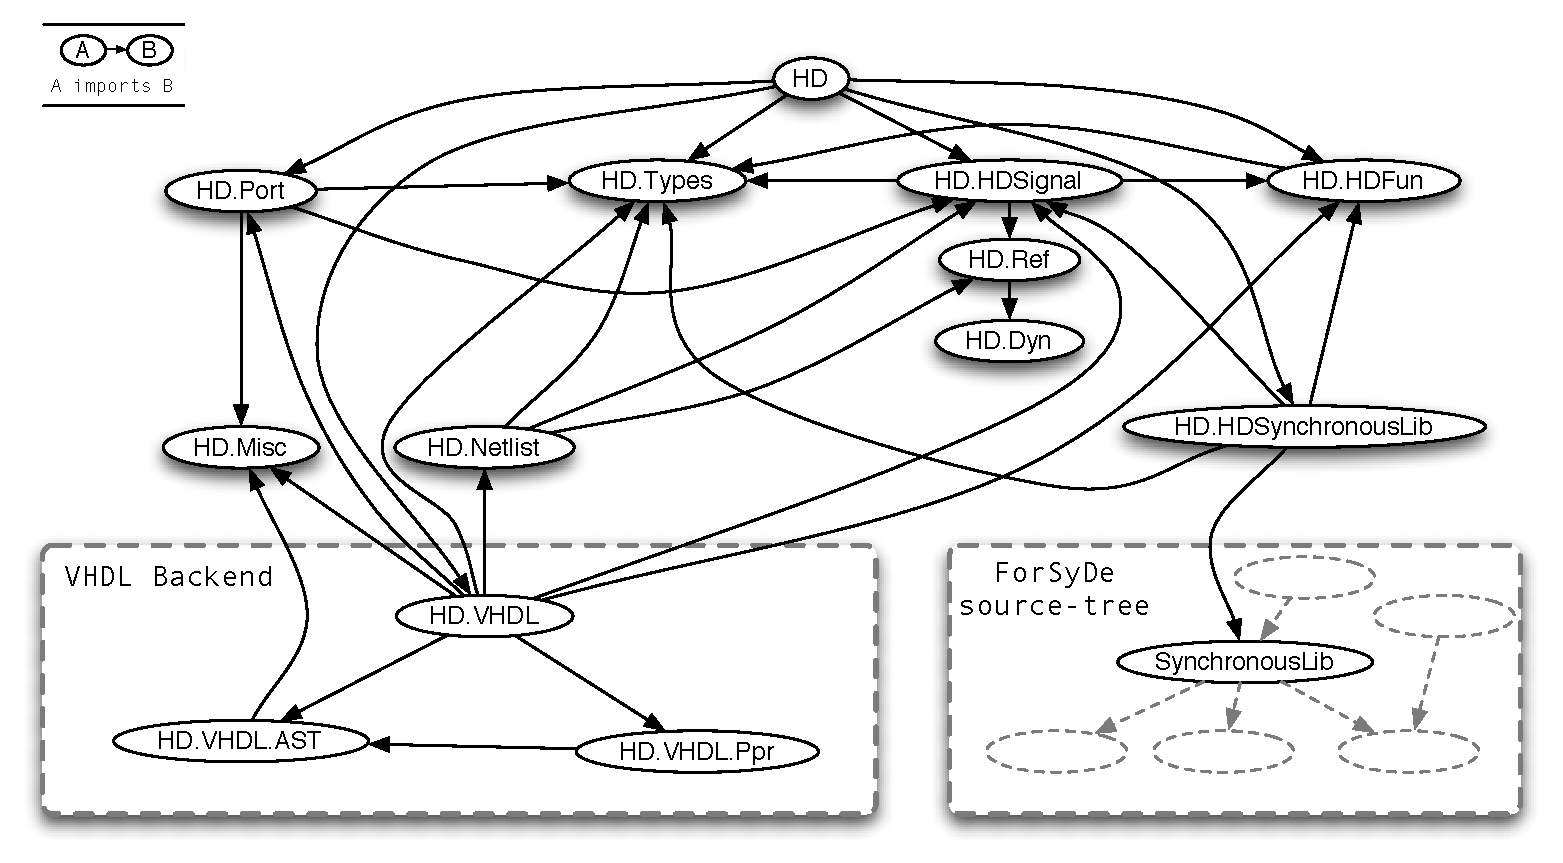
\includegraphics[height=.8\textwidth]{graph.pdf}
  \caption{Compiler modules' dependency graph}
  \label{fig:graph}
\end{figure}
\end{landscape}


\item \texttt{\textbf{HD.HDSignal}}. It is, without doubt, the most important
  module. It contains the definition of the user-hidden
  \textit{Hardware Description Signal}. 


  
  As it was previously mentioned, an \texttt{HDSignal}
  \textit{secretly} stores the structure of the circuit for latter
  processing, it is the compiler's intermediate representation of a
  circuit-description, and thus, it is the only usable information
  which a backend can work with.

  An \texttt{HDSignal} uses the same signal approach as
  Lava \cite{lava}, called \textit{Observable Sharing} \cite{osharing}
  which was earlier introduced in chapter \ref{chap:vs}.  Actually,
  both the modules \texttt{\textbf{HD.Ref}} (the Observable Sharing
  implementation) and \texttt{\textbf{HD.Dyn}} (unsafe dynamic types,
  used internally in \texttt{HD.Ref}) were taken and adapted from the
  Lava distribution.

  It is encouraged to fully understand the details of this module before
  attempting to extend the compiler or even trying to understand any other
  part of the source tree.

\item \texttt{\textbf{HD.HDFun}}. Most of the ForSyDe process
  constructors, such as $\mathit{mapSY}$ (see chapter
  \ref{chap:intro}) are represented in terms of a higher order
  function. That is, a function is passed along with the signal in
  order process it.
  
  The syntactical information of those functions needs to be
  internally stored (bundled with an \texttt{HDSignal}) for latter
  translation to the target language. The \texttt{HD.HDFun} module
  makes use of Template Haskell to make it possible: It provides a
  data structure (\texttt{HDFun}) which stores all the function
  information and a constructor (\texttt{mkHDFun}) to create such
  structure from the Template-Haskell representation
  (~\texttt{Q[Dec]}) of a function.  Colaterally, \texttt{HD.HDFun} is
  responsible of establishing the Haskell syntax-subset supported by
  \texttt{HDFun}s.

  Familiarity with Template Haskell is obviously a must in order to
  deal with this module.
\end{itemize}

\subsection{Miscellaneous auxiliary functions and types}

\texttt{\textbf{HD.Misc}} contains miscellaneous helper functions and
types which are too small to be splitted in their own modules.  The
only important part to highlight is the \texttt{EProne a} type, which
holds an \textit{error-prone} value and uses \texttt{mtl}'s
\texttt{Error} monad class to handle those errors.
  
Error management within the compiler is handled, to a large extend,
through the \texttt{Eprone} type.

\subsection{Ports, Blocks and Block Instances}
The concepts of a \textit{Port},\textit{Block} and \textit{Block
  Instance} were introduced in chapter \ref{chap:design}. The
\texttt{HD.Port} module implements them and enables their use,
providing as well an API to the end-user to deal with them.

The introduction of Ports has implied as well the introduction of
typecheking (there is no way to statically assure whether a the type
of a port entry matches a signal attached to it).

Moreover, due to the fact that the compiler is Embedded in Haskell,
compilation of the guest language (i.e. ForSyDe models) strangely
takes place at runtime, and unavoidably so does typechecking. 

As a result, the functions which attach or obtain signals to/from a
port (namely \texttt{plugSig} and \texttt{supplySig}) are in charge of doing
typechecking.

Moreover, due to the restrictions imposed by the host language,
typechecking turns to be a difficult task. A tricky solution using
dynamic signals (that is, \texttt{forall}\footnote{If you are confused
  with the \texttt{forall} keyword, that means you should 
  get familiar with existential types before trying to go through this
  module.}\texttt{a.HDPrimType a => HDSignal a}) was figured out. It
works nicely in practice, but it certainly could (and probably should)
be redesigned or improved.

The coexistence of static and dynamic signals requires a way of
conversion between them. That is the purpose of the \texttt{sigCast} function.

\subsection{Backends}
\label{backends}
A backend is in charge of interpreting the intermediate representation
of the source code. The most common form of interpretation is a
translation into another language (e.g.  \texttt{VHDL}) but some other
possibilities are: simulation, design verification, generation of a graphical
representation etc $\dots$. 

In our case, a backend uses a \texttt{Block} as input, whose netlist
(the internal circuit graph) is traversed to achieve the
aforementioned interpretation. 

The module \texttt{HD.NetList} (which was imported and adapted from
Lava) provides the developer with \texttt{netlist}, a function which
carries out the traversal of the circuit. Due to the use of
\textit{Observable Sharing} in the circuit representation, which is
right now is restricted to \texttt{IO}-references (see module
\texttt{HD.Ref}) \texttt{netlist} is subdued to the \texttt{IO} Monad.
Furthermore, in order to allow reading and modifying state data during
the traversal, the \texttt{IO} Monad is wrapped into \texttt{mtl}'s
\texttt{StateT} monad transformer.

There could be interpretations, such as simulation, for which a
\texttt{ST} version of \texttt{netlist} would be preferable to current
\texttt{IO} version. Adding an alternative \texttt{ST} version would
involve including \texttt{ST}-references in \texttt{HD.Ref} (maybe
from the Lava-project, which already offers them).

Currently, the only available backend is a translator to VHDL, which
is divided in three modules

\begin{itemize}
\item \texttt{\textbf{HD.VHDL}}. It is in charge of the VHDL translation,
  which is accessible through the \texttt{writeVHDL} function.

\item \texttt{\textbf{HD.VHDL.AST}} defines data structures to hold
  the AST (\textit{Abstract Syntax Tree}) of the generated VHDL modules.  

  It is based in the grammar of the VHDL93 standard but only supports
  the subset of VHDL's syntax which has been needed. However, due to
  being based in the standard it could be easily extended in the
  future if desired.
  
\item \texttt{\textbf{HD.VHDL.Ppr}}. A \texttt{pretty-printer} library
  for the VHDL AST-structures mentioned above. It is in charge of the
  transformation and output of the AST into readable VHDL text
  modules.

\end{itemize}

\subsection{Integration with ForSyDe}

The development of the compiler did not entail big changes in
the ForSyDe library. A new alternative signal type (\texttt{HDSignal})
was developed to avoid modifying ForSyDe's original stream-based
\texttt{Signal} type.

However, one of the main compiler design-requirements was to be able
to reuse the original name and semantics of ForSyDe's
signal-processing functions with the new signal type.  It is a
certainly nice feature, since it allows all earlier documentation to
still apply for both signal types. In order to make it possible,
ForSyDe's original \texttt{SynchronousLib} module had to be modified.
Its \texttt{mapSY}, \texttt{zipWithSY} and \texttt{delaySY} functions
(the only ForSyDe processes currently supported natively by the
compiler) were transformed into type classes\footnote{Due to the
  nature of the the signal processing functions, the type classes
  required various parameters, and thus \textit{Multiparameter Type
    Classes} (a common Haskell extension) where used for that
  purpose.} and instances were created for both \texttt{Signal} and
\texttt{HDSignal}.

The new type classes and \texttt{Signal} instances remain in
\texttt{SynchronousLib} while the \texttt{HDSignal} ones were included
in a new module: \texttt{HDSynchronousLib}.

It is worth to note that, even if the compiler only currently supports
$\mathit{mapSY}$, $\mathit{zipWithSY}$ and $\mathit{delaySY}$ natively
as primitives\footnote{It can be said that they constitute the
  primitive processes of the compiler.}, due to the type class scheme
described above, all their derived process constructors (e.g.
$\mathit{sourceSY}$), are automatically supported.  However they are
treated as compound processes and thus, there is currently no way to
internally identify them as individual entities.  Treating those
derived processes as primitives would be desirable for a more precise
control of the way in which the design is interpreted, allowing
optimizations and improving code generation in the backends.

\section{Recipes to extend the compiler}

The following sections are targeted at suggesting the steps to follow
when developing common extensions for the compiler. 

The main purpose of these recipes is to help new developers, only
interested in certain extensions, to get familiar with the compiler.
Depending on the extension, some other changes might be required. As a
result, it is encouraged to take the recipes with a grain of salt and
expect further modifications to be needed in the process.

\subsection{Adding support for new types of signal values}

\texttt{Bool} and \texttt{Int} \texttt{HDSignal}s might be enough for
many designs, but it can be a good idea to support other signal values such as
tuples, enumerates etc $\dots$

To add a new type, say \texttt{a}

\begin{enumerate}[1)]
\item Add a constructor for \texttt{a} in \texttt{HD.HDTypes.HDType}
\item Make \texttt{a} an instance of \texttt{HD.HDTypes.HDPrimType}
\item Add a constructor for \texttt{a} in \texttt{HD.HDTypes.HDPrimConst}
\item Adjust the backends to handle the new type. In the VHDL backend
  that roughly means changing \texttt{HD.VHDL.hDST2TM} and
  \texttt{HD.VHDL.hDPC2Expr}.
\item The new type might require extending the Haskell subset
  supported by \texttt{HDFun}s. For instance, tuples would be difficult to
  use without pattern matching. Read on for details about how to perform
  this extension.
\item Consider adding support for new functions within an
  \texttt{HDFun}.  As an example, in the case of choosing to add
  support for tuples, it would be desirable to get support for
  well-known \texttt{fst} and \texttt{snd} functions.  Details about
  how to do this are covered in a following section.
\end{enumerate}

\subsection{Treating more ForSyDe processes as primitives}

As it was previously stated, the only process constructors treated
natively as primitives are $\mathit{mapSY}$, $\mathit{zipWithSY}$ and
$\mathit{delaySY}$.  $\mathit{sourceSY}$, for example, is handled as a
compound of $\mathit{mapSY}$ and $\mathit{delaySY}$.

In order to treat a process, say $\mathit{sourceSY}$ from ForSyDe's
original \texttt{SynchronousLib}, as a primitive:

\begin{enumerate}[1)]
\item Add \texttt{sourceSY} to \texttt{HD.HDSignal.HDSignal}
\item Transform \texttt{SynchronousLib.sourceSY} into a type class and use
  its previous definition to make \texttt{Signal} an instance of it.
\item Modify \texttt{HD.HDSynchronousLib} by making \texttt{HDSignal}
  an instance of the new \texttt{SourceSY} class.
\item Adjust the backends to handle the new primitive. Basically, that entails
  changing the \texttt{new} and \texttt{define} functions passed to
  \texttt{netlist}, see \texttt{HD.VHDL} for more details.
\end{enumerate}

\subsection{Extending \texttt{HDFun}'s Haskell-syntax subset}
The Haskell syntax admited by \texttt{HDFun}s (more precisely by
\texttt{HD.HDFun.mkHDFun}) is quite limited. For example, neither
constructor pattern-matching nor \textit{where-clauses} are allowed
(chapter \ref{chap:design} gives a precise description of the supported
subset).

To broaden the supported Haskell-subset.

\begin{enumerate}[1)]
\item Locate what type in the the Template Haskell AST
  (\texttt{Language.Haskell.TH.Syntax}) holds the desirable syntax
  extension.
\item Modify the corresponding \texttt{Lift} instantiate for that type in
  \texttt{HD.HDFun}  in order to give support to the new feature.
\item Adapt the compiler backends to the change.
\end{enumerate}
 
\subsection{Adding support for new functions within \texttt{HDFun}s}
The functions which a designer can use within a \texttt{HDFun} (e.g.
\texttt{(\&\&)}, \texttt{(==)}, \texttt{(-)}, \texttt{(+)} $\dots$ )
are limited.  That limitation, however, is not intrinsic to
\texttt{HDFun}s themselves, which can indeed make use of any valid
Haskell function as long as it is done in a correct manner. The
problem is that those functions have to be interpreted at some point
by the translation backends.

Thus, in order to support new functions within an \texttt{HDFun}, the
backend has to be aware of them and know how to handle them.
For that reason, to add in a new function simply ...

\begin{itemize}
\item Adapt the backends to support the new function.
\end{itemize}

The way to dispatch those functions depends highly on the translation
backend, for example, in the \texttt{VHDL} backend, translation tables
are kept to help mapping them from Haskell to VHDL.

A simulation backend on the other hand does not involve a translation
and could make use of the original Haskell function (which is stored
in the \texttt{HDFun} algebraic type). That makes possible to forget
about the \texttt{HDFun} AST and translation tables.

\subsection{Adding a new backend}

To add a new backend such as simulation, translation to another target
language or code verification, the intermediate representation the ForSyDe
model has to be traversed and processed. A good way to start up would be
looking at the sources of current \texttt{VHDL} backend to understand how the
\texttt{netlist} function works in practice.

A simulation backend could be coded as follows.

\begin{enumerate}[1)]
\item Verify whether the \texttt{HD.NetList.netlist} function fulfils
  the needs of the backend and otherwise create an alternative version.

  Simulation could serve as a means of translating between
  \texttt{HDSignal}s and \texttt{Signal}s but unfortunately
  \texttt{netlist} depends on \texttt{IO} from which no one can safely
  escape (transforming an \texttt{IO a} value into \texttt{a} 
  causes side effects). Thus, a
  \texttt{ST}-\texttt{netlist}\footnote{The \texttt{a} value of
    \texttt{ST a} can be extracted through \texttt{runST}} version
  would be necessary to bypass \texttt{IO}.  See section
  \ref{backends} for more details.

\item Check if the intermediate representation of the circuit
  (contained in \texttt{\texttt{HD.\-HDSignal.\-HDSignal}}) needs to
  be extended.
  
  A simulation backend would need to make use of the original Haskell
  function stored in \texttt{HDFun}s to avoid having to traverse its
  AST. However, the function itself is not stored in an \texttt{HDSignal}

\item Lastly, code the backend.
\end{enumerate}

\section{Improving the source code}

Every piece of software is an evolving entity which can always be
improved. The compiler produced during this thesis is no exception and
is far for being perfect in many ways.

Due to the time-limitation of the thesis, I was not able to make the
code be organized and work as good I would have liked to, but at least
I was careful enough to anotate and coment all the potential
improvements I could notice.  I used the traditional \texttt{FIXME}
and \texttt{TODO} tags for that purpose.

Reading the output produced by \texttt{grep -ri 'TODO$\backslash$|FIXME' *} in
the \texttt{HD} directory gives a good hint about where to start
working.



\chapter{Examples}
\label{chap:examples}
\section{$\mathit{plus1}$}

\subsection{\texttt{Plus1.hs}}
ForSyDe specification model of a simple adder system.
 
\lstinputlisting[language=haskell]{B.Examples/Plus1.hs}
\clearpage
\subsection{\texttt{plus1.vhd}}
VHDL code generated from its Haskell model. Note that the code depends
on ForSyDe's VHDL Library, which is included in appendix
\ref{chap:vhdllib}.

\lstinputlisting[language=VHDL]{B.Examples/plus1.vhd}
\newpage
\subsection{RTL model of $\mathit{plus1}$}
RTL model obtained with Altera's \textit{Quartus II} software after
compiling the VHDL model for a Stratix FPGA.

\begin{figure}[h]
\centering
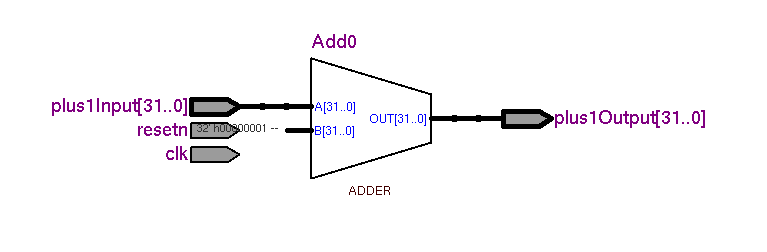
\includegraphics[scale=.7]{plus1.png}
\caption{RTL model of $\mathit{plus1}$}
\end{figure}


\chapter{ForSyDe's VHDL Library}
\label{chap:vhdllib}
\section{\texttt{forsyde.vhd}}
The following listing conatins the, still very simple, source code of
\texttt{forsyde.vhd}, a VHDL library used by the target VHDL
models.  

\lstinputlisting[language=VHDL]{../../lib/forsyde.vhd}


\nocite*
\bibliography{report}
\bibliographystyle{unsrt}
  
\end{document}

